\documentclass[utf8, a4paper, 11pt, envcountsect]{beamer}

\usepackage[english]{babel}
\usepackage[T1]{fontenc}

\usepackage{amsmath, amsfonts, wrapfig, graphicx}
\usepackage{bm}
\usepackage{mathtools}
\usepackage{stmaryrd}

\usepackage{beamerthemesplit}
\usetheme{CambridgeUS}

\setbeamertemplate{footline}
{\leavevmode%
  \hbox{%
  \begin{beamercolorbox}[wd=\paperwidth,ht=2.25ex,dp=1ex,right]{date in head/foot}%
    \usebeamerfont{date in head/foot}\insertshortdate{}\hspace*{2em}
    \insertframenumber{}-\inserttotalframenumber\hspace*{2ex} \end{beamercolorbox}}%
}

\setbeamertemplate{navigation symbols}{}  % Remove navigation bear
\setbeamertemplate{theorems}[numbered]

\newtheorem{innercustomgeneric}{\customgenericname}
\providecommand{\customgenericname}{}
\newcommand{\newcustomtheorem}[2]{%
  \newenvironment{#1}[1]
  {%
   \renewcommand\customgenericname{#2}%
   \renewcommand\theinnercustomgeneric{##1}%
   \innercustomgeneric}
  {\endinnercustomgeneric}
}

\newcustomtheorem{thm}{Theorem}
\newcustomtheorem{lem}{Lemma}
\newcustomtheorem{cor}{Corollary}
\newcustomtheorem{deftn}{Definition}
\newcustomtheorem{prop}{Proposition}
%\newtheorem{prop}{Proposition}
\DeclareMathOperator*{\argmin}{argmin}
\DeclareMathOperator*{\dist}{dist}
\DeclareMathOperator*{\argmax}{argmax}
\DeclareMathOperator*{\Tr}{Tr}

\title{General ideas on interpolation}
\institute[Uhlmann's lab]{\textbf {V. Uhlmann's lab}}
\author{Yoann Pradat}
\date{\today}
\titlegraphic{
\includegraphics[width=4cm]{EMBL_EBI-logo.png}}

\begin{document}


\frame{\titlepage}

\section[Outline]{}
\frame{\tableofcontents}

\section{Introduction}

\frame{\frametitle{Objective}
  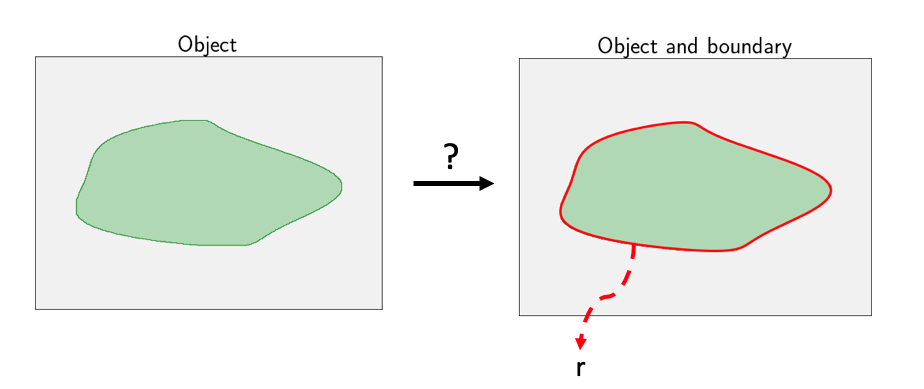
\includegraphics[width=0.9\linewidth]{motivation.png}

  \underline{Objective}: find mathematical model for the \textbf{boundary} 
  
  \begin{equation}
    {\bf r} = \begin{bmatrix} r_1 \\ \vdots \\ r_d \end{bmatrix}
  \end{equation}

}

\frame{\frametitle{Generic model}
  \begin{equation}
    {\bf r}(t) = \begin{bmatrix} r_1 \\ \vdots \\ r_d \end{bmatrix} = \sum_{k \in \mathbb{Z}} \begin{bmatrix} c_1(k) \\ 
    \vdots \\ c_d(k) \end{bmatrix} \phi_k(t)
  \end{equation}
  \underline{Vocab}
  \begin{itemize}
    \item ${(t_k=k)}_{k \in \mathbb{Z}}$ \textbf{knots} locations
    \item ${\bf c}(k) := \begin{bmatrix} c_1(k) \\ \vdots \\ c_d(k) \end{bmatrix}$ are \textbf{control points}
    \item ${(\phi_k)}_{k \in \mathbb{Z}} :=$ set of \textbf{basis functions} or \textbf{generators}
  \end{itemize}
}

\frame{\frametitle{Impact of varying ${\bf c}(k)$}
  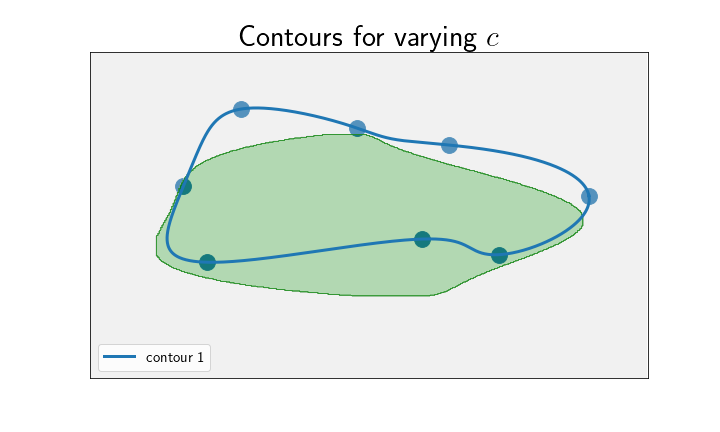
\includegraphics[width=\linewidth]{example_var_c_1.png}
}

\frame{\frametitle{Impact of varying ${\bf c}(k)$}
  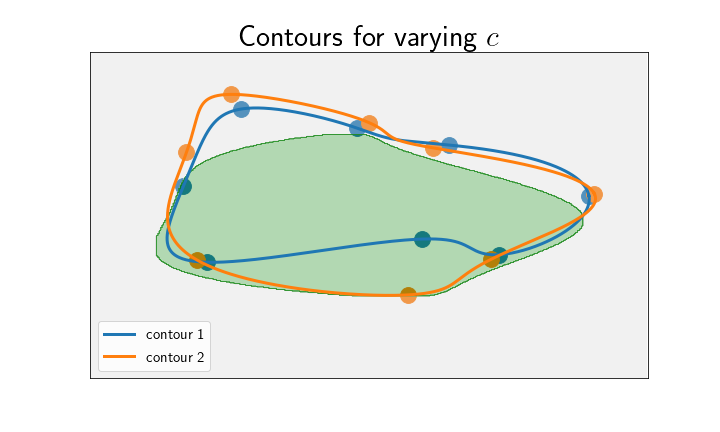
\includegraphics[width=\linewidth]{example_var_c_2.png}
}

\frame{\frametitle{Impact of varying ${\bf c}(k)$}
  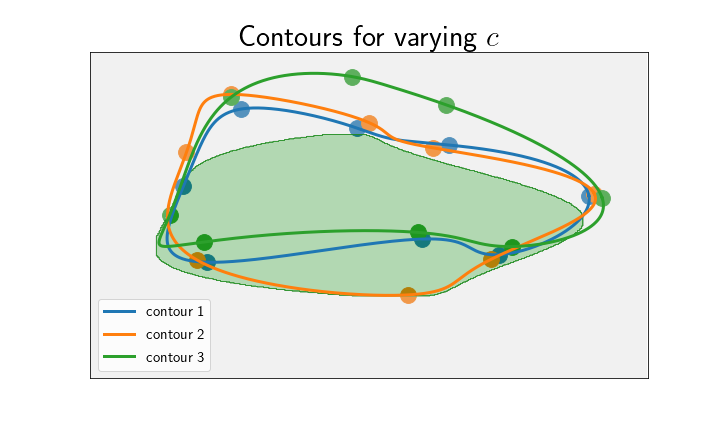
\includegraphics[width=\linewidth]{example_var_c_3.png}
}

\frame{\frametitle{Impact of varying ${\bf c}(k)$}
  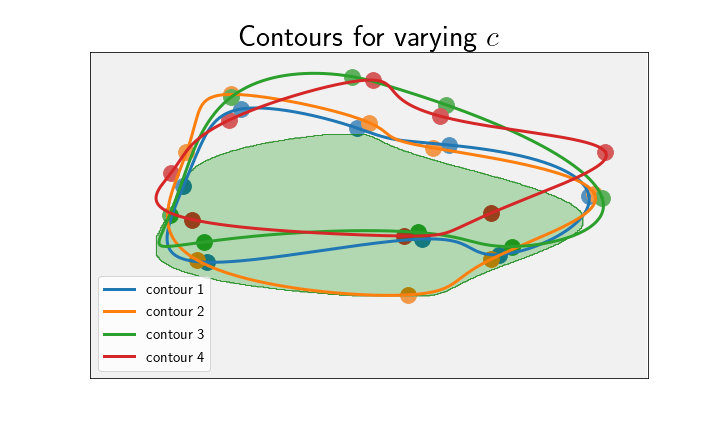
\includegraphics[width=\linewidth]{example_var_c_4.png}
}

\frame{\frametitle{Impact of varying $\phi_k$}
  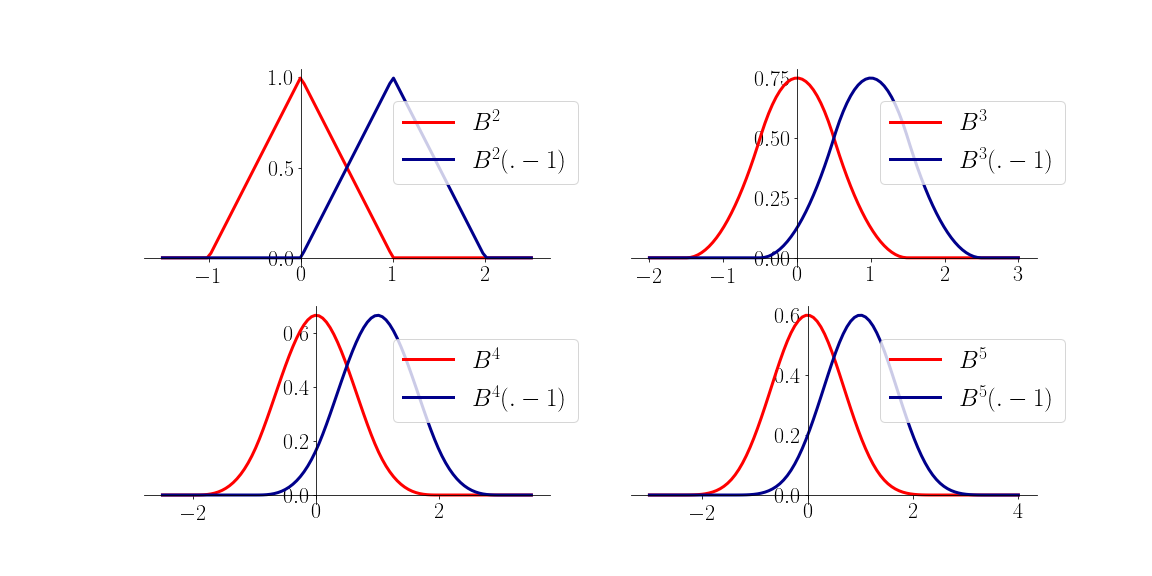
\includegraphics[width=\linewidth]{example_bspline.png}
  \begin{equation*}
    {(\phi_k)}_{k \in \mathbb{Z}} = {(\tau_k B)}_{k \in \mathbb{Z}} \quad \text{with} \quad \tau_k f = f(.-k)
  \end{equation*}
}

\frame{\frametitle{Impact of varying $\phi_k$}
  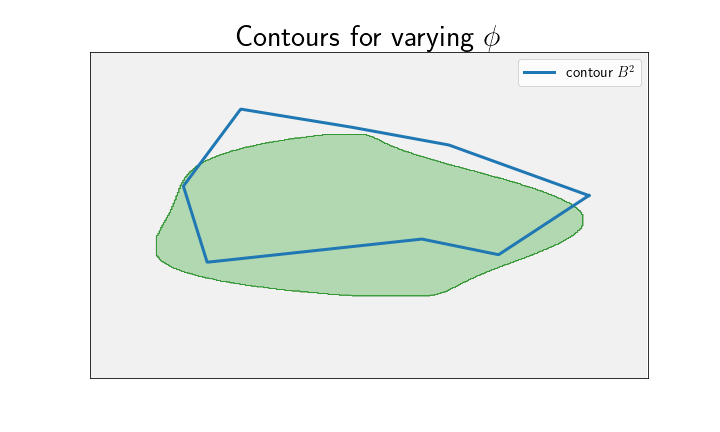
\includegraphics[width=\linewidth]{example_var_b_1.png}
}

\frame{\frametitle{Impact of varying $\phi_k$}
  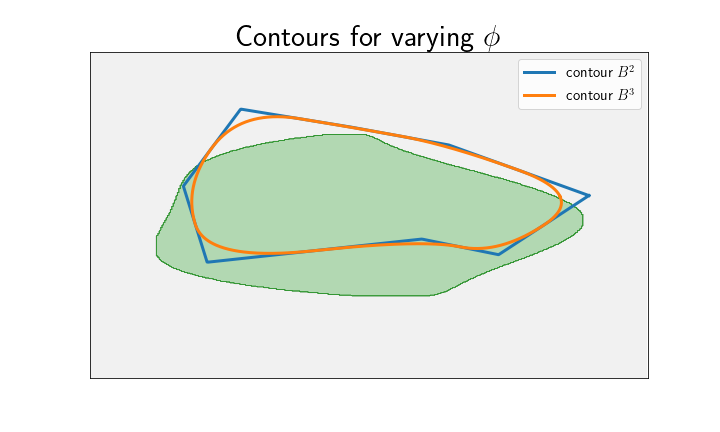
\includegraphics[width=\linewidth]{example_var_b_2.png}
}

\frame{\frametitle{Impact of varying $\phi_k$}
  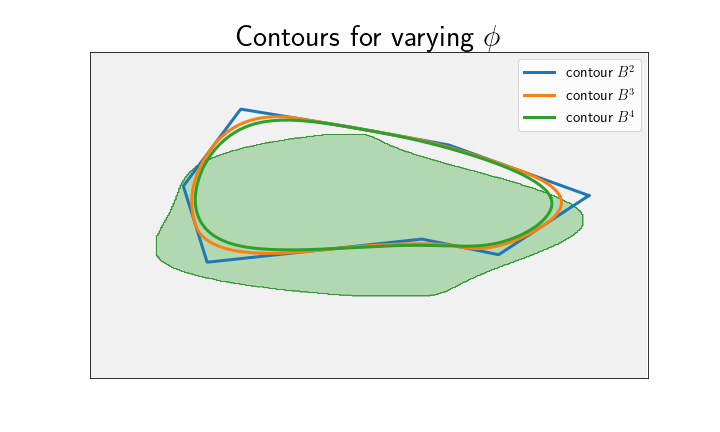
\includegraphics[width=\linewidth]{example_var_b_3.png}
}

\frame{\frametitle{Impact of varying $\phi_k$}
  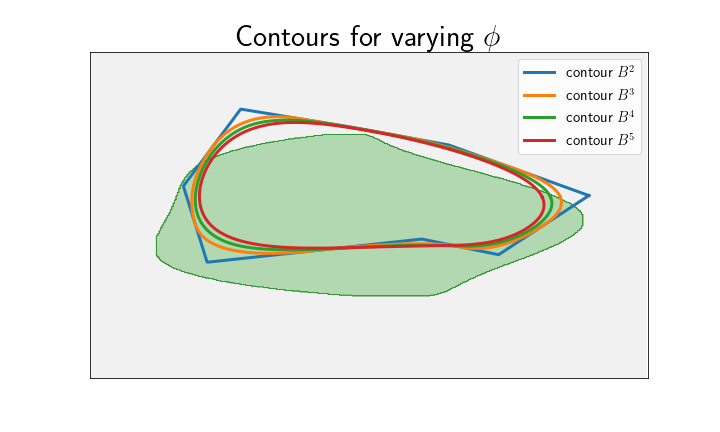
\includegraphics[width=\linewidth]{example_var_b_4.png}
}

\frame{\frametitle{Approximation, interpolation}
  \underline{Boundary approximation} Fixed generators $\phi_k$, optimize the values of ${\bf c}(k)$.
  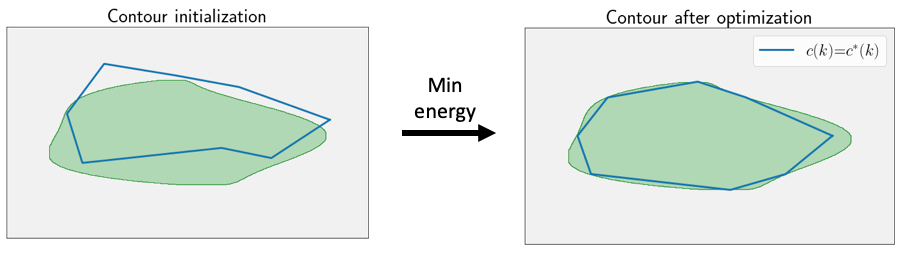
\includegraphics[width=0.95\linewidth]{example_energ.png}
  \pause%
  \underline{Feedback?} Intuitive understanding of control points
  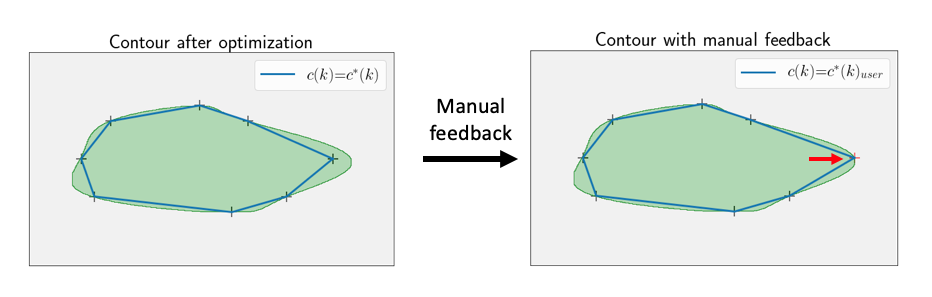
\includegraphics[width=0.95\linewidth]{example_user.png}
}

\frame{\tableofcontents}

\section{I/ Polynomial interpolation}
\subsection{I/1 Principles}

%%%%%%%%%%%%%%%
%% FRAME 1
%%%%%%%%%%%%%%%

\frame{\frametitle{Lagrange polynomials}
  \underline{Not.}
  \begin{itemize}
    \itemsep0em
    \item $\Pi_{<n} = \{p \in \mathbb{R}[X] | \deg(p) \leq n-1\}$
    \item $t_1 < \cdots < t_n$
  \end{itemize}
  \underline{Obj}: reconstruct $g:\mathbb{R} \to \mathbb{R}$ from $g(t_1), \ldots, g(t_n)$.  
  
  \begin{prop}{1 (Lagrange 1795)}
    $\exists!f \in \Pi_{<n}$ s.t $\forall i=1,n$, $f(t_i)=g(t_i)$
  \end{prop}
  \pause%
  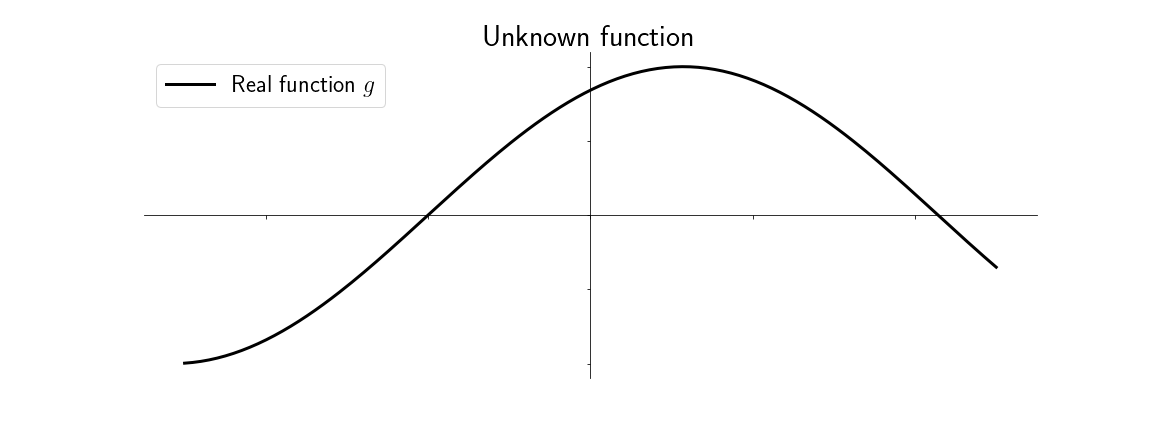
\includegraphics[width=0.9\linewidth]{lagrange_1.png}
}

\frame{\frametitle{Lagrange polynomials}
  \underline{Not.}
  \begin{itemize}
    \itemsep0em
    \item $\Pi_{<n} = \{p \in \mathbb{R}[X] | \deg(p) \leq n-1\}$
    \item $t_1 < \cdots < t_n$
  \end{itemize}
  \underline{Obj}: reconstruct $g:\mathbb{R} \to \mathbb{R}$ from $g(t_1), \ldots, g(t_n)$.  
  
  \begin{prop}{1 (Lagrange 1795)}
    $\exists!f \in \Pi_{<n}$ s.t $\forall i=1,n$, $f(t_i)=g(t_i)$
  \end{prop}
  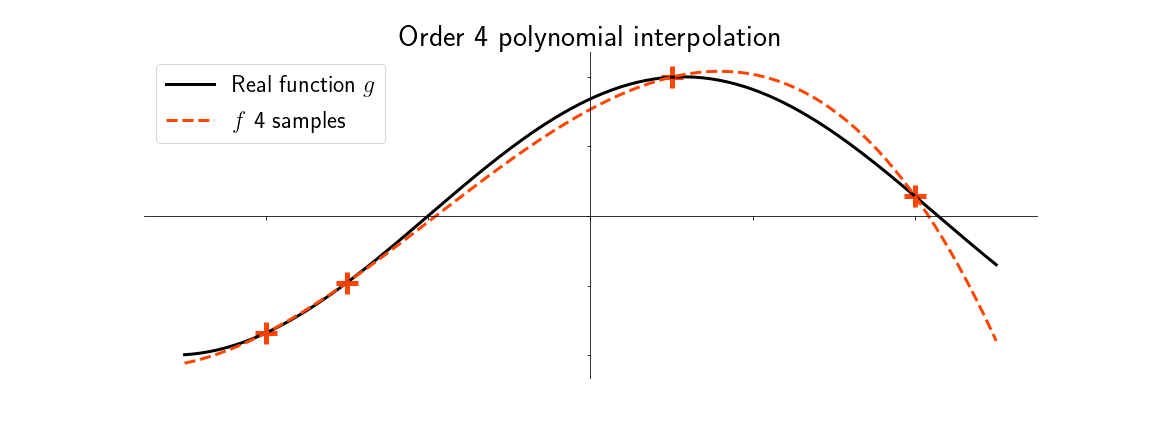
\includegraphics[width=0.9\linewidth]{lagrange_2.png}
}

\frame{\frametitle{Lagrange polynomials}
  \underline{Not.}
  \begin{itemize}
    \itemsep0em
    \item $\Pi_{<n} = \{p \in \mathbb{R}[X] | \deg(p) \leq n-1\}$
    \item $t_1 < \cdots < t_n$
  \end{itemize}
  \underline{Obj}: reconstruct $g:\mathbb{R} \to \mathbb{R}$ from $g(t_1), \ldots, g(t_n)$.  
  
  \begin{prop}{1 (Lagrange 1795)}
    $\exists!f \in \Pi_{<n}$ s.t $\forall i=1,n$, $f(t_i)=g(t_i)$
  \end{prop}
  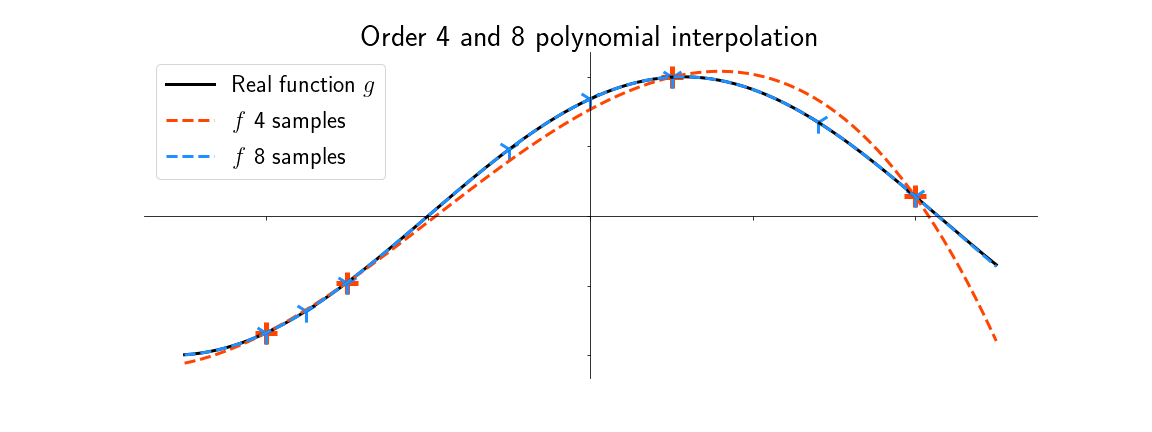
\includegraphics[width=0.9\linewidth]{lagrange_3.png}
}

%%%%%%%%%%%%%%%
%% FRAME 2
%%%%%%%%%%%%%%%

\frame{\frametitle{Osculatory interpolation}
  \underline{Not.}
  \begin{itemize}
    \itemsep0em
    \item $f$ agrees with $g$ at $\underbrace{(t, \dots, t)}_{\text{$r$ times}}$ if $\forall m \in \llbracket 0, r-1 
      \rrbracket, f^{(m)}(t) = g^{(m)}(t)$
    \item $t_1 = \cdots = t_{r_1} \leq \cdots \leq t_{r_1 + \cdots + r_{d-1}+1} = \cdots = t_{r_1 + \cdots + r_d}$ with 
      $d$ unique
  \end{itemize}
  \begin{prop}{2 (Consequence theorem 1)}
    $\exists!f \in \Pi_{<n}$ s.t $\forall i \in \llbracket 0, d \rrbracket$, $f(t_i)=g(t_i), \ldots, 
    f^{(r_i-1)}(t_i)=g^{(r_i-1)}(t_i)$
  \end{prop}
}

%%%%%%%%%%%%%%%
%% FRAME 3
%%%%%%%%%%%%%%%

\frame{\frametitle{Divided differences}
  \underline{Not.}
  \begin{itemize}
    \itemsep0em
    \item $t_1 \leq \cdots \leq t_n$ with $d$ unique
  \end{itemize}
  \begin{deftn}{1}
    $[t_1, \dots, t_n]g$ leading coeff of $f \in \Pi_{<n}$ s.t $f(t_i) = g(t_i)$
  \end{deftn}
  \underline{Examples} 
  
  \begin{enumerate}
    \item $[t_1]g = g(t_1)$
    \item $[t_1, t_2]g =\left\{
      \begin{array}{@{}ll@{}}
    \frac{g(t_2)-g(t_1)}{t_2-t_1} & \text{if}\ t_1\neq t_2 \\
    g'(t_1), & \text{otherwise}
  \end{array}\right.$
  \end{enumerate}
  \pause%
  \begin{small}
  \begin{prop}{3}
    \begin{enumerate}
      \item if $g \in\mathcal{C}^{(n-1)}$, $\exists\eta\in[t_1, t_n]$ s.t $[t_1, \dots, t_n]g = \frac{g^{(n-1)} 
        (\eta)}{n!}$
      \item $f \in\Pi_{<n}$ s.t $f (t_i) = g (t_i)$ is $f (t) = \sum_{i=1}^n (t-t_1)\dots(t-t_{i-1})[t_1, \dots, t_i]g$.
      \end{enumerate}
  \end{prop}  
\end{small}
}

%%%%%%%%%%%%%%%
%% FRAME 4
%%%%%%%%%%%%%%%

\frame{\frametitle{Osculatory theorem}
  \underline{Not.}
  \begin{itemize}
    \itemsep0em
    \item $t_1 \leq \cdots \leq t_n$ with $d$ unique
  \end{itemize}
  \begin{thm}{1 (C. De Boor 1978)}
  Let $g \in \mathcal{C}^{(n)}$. Then $\forall t$, $g = f_n + (t-t_1)\dots(t-t_n)[t_1, \dots, t_n, t]g$.
  \end{thm}
  \pause%
  \underline{Example}
  \begin{itemize}
    \item $t_1=\cdots=t_n$, $\displaystyle g(t) = \sum_{i=0}^{n-1}  \frac{g^{(i)}(t_1)}{i!} {(t-t_1)}^i  + 
      \frac{g^{(n)}(\eta_t)}{n!} {(t-t_1)}^n$
  \end{itemize}

}

\subsection{I/2 Limits}


%%%%%%%%%%%%%%%
%% FRAME 5
%%%%%%%%%%%%%%%


\frame{\frametitle{Runge: high-order interpolation can be bad}
  \underline{Not.}
  \begin{itemize}
    \item $t_1 < \cdots < t_n$ uniform on $[-1,1]$
    \item $g(t) = \frac{1}{1+25t^2}$
  \end{itemize}
    \pause%
  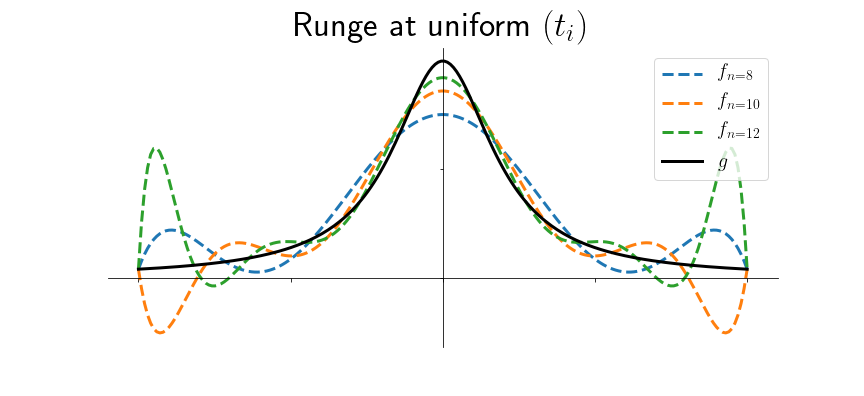
\includegraphics[width=\linewidth]{runge_1.png}
}


%%%%%%%%%%%%%%%
%% FRAME 6
%%%%%%%%%%%%%%%


\frame{\frametitle{Runge explained}
  \underline{Not.}
  \begin{itemize}
    \itemsep0em
    \item $a=t_1 < \cdots < t_n=b$
    \item $\| f \| = {\|f\|}_{\infty, [a,b]} = \sup_{a \leq t \leq b} |f(t)|$
    \item $\displaystyle f_n = \sum_{i=1}^n g(t_i) \phi_i$, $\phi$ Lagrange pol.
    \item $\lambda_n(t) = \sum_{i=1}^n |\phi_i(t)|$
  \end{itemize}
  \pause%
  \underline{Magnitude interpolator}
  \begin{align*}
    \text{For} \quad t_i \leq t \leq t_{i+1}, |f_n(t)| & \leq \sup_{1 \leq i \leq n} |g(t_i)| |\lambda_n(t)| \\
    & \leq \|g\| \|\lambda_n\| \\
    \text{hence} \quad \|f_n\| & \leq \|g\| \|\lambda_n\|
  \end{align*}

  \begin{itemize}
    \item Bound is sharp
    \item  Uniform $(t_i) \implies \|\lambda_n\| \sim \frac{2^n}{en \log(n)}$.
  \end{itemize}
}


%%%%%%%%%%%%%%%
%% FRAME 7
%%%%%%%%%%%%%%%

\frame{\frametitle{Chebyshev sites are good}
  \underline{Not.}
  \begin{itemize}
    \itemsep0em
    \item $a=t_1 < \cdots < t_n=b$
    \item $\| f \| = {\|f\|}_{\infty, [a,b]} = \sup_{a \leq t \leq b} |f(t)|$
    \item $g \in \mathcal{C}^{(n)}[a,b]$
  \end{itemize}
  \pause%
  \underline{Analysis of the error}
  \begin{align*}
    \text{Osculatory thm} \quad |g(t)-f_n(t)| &= |(t-t_1) \dots (t-t_n)[t_1, \dots, t_n, t]g| \\
    &\leq \|(.-t_1) \dots (.-t_n)\| \frac{\|g^{(n)}\|}{n!}
  \end{align*}
  \pause%
  \underline{Idea}: take $(t_i^c) = \argmin_{a \leq t_1 \leq \cdots \leq t_n \leq b} \|(.-t_1) \dots (.-t_n)\|$
  \begin{enumerate}
    \item $t_i^c = [(a+b) - (a-b) \cos (\frac{(2i-1)\pi}{2n})]/2$
    \item $\|(.-t_1^c) \dots (.-t_n^c)\| = 2{\left(\frac{b-a}{4}\right)}^n$
  \end{enumerate}
 }


%%%%%%%%%%%%%%%
%% FRAME 8
%%%%%%%%%%%%%%%

\frame{\frametitle{Jackson's theorem}
  \underline{Not.}
  \begin{itemize}
    \itemsep0em
    \item $w(g, h) = \sup \{ |g(t)-g(s)|, |t-s| \leq h\}$
  \end{itemize}

  \begin{thm}{2}
    If $g \in \mathcal{C}^{r}([a..b])$ and $n > r+1$ then
    \begin{equation}
      \dist(g, \Pi_{<n}) \leq const_r {\left(\frac{b-a}{n-1}\right)}^r w(g^{(r)}, \frac{b-a}{2n-1-r})
    \end{equation}
  \end{thm}
  \pause%

  \textbf{Idea}: break interval $[a,b]$ into pieces. \\

  \begin{itemize}
    \item \underline{Pros} low order polynomials
    \item \underline{Cons} continuity at break points
  \end{itemize}
}

\section{II/ Piecewise-polynomial interpolation}
\frame{\tableofcontents}

\subsection{II/1 Piecewise-linear}

%%%%%%%%%%%%%%%
%% FRAME 9 
%%%%%%%%%%%%%%%

\frame{\frametitle{Interpolator $I_2$}
  \underline{Not.}
  \begin{itemize}
    \itemsep0em
    \item $a=t_1 < \cdots < t_n=b$, $g: [a,b] \to \mathbb{R}$
    \item $\Pi_{<n, {\bf t}} = \{\text{pp of order $n$ with breaks at $t_2, \ldots, t_{n-1}$}\}$
    \item $\$_{2, {\bf t}} = \Pi_{<2, {\bf t}} \cap \mathcal{C}^0$
  \end{itemize}
  \pause%
  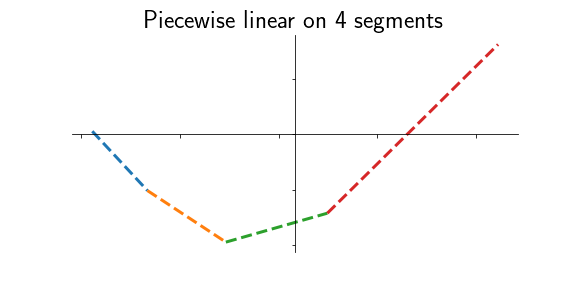
\includegraphics[width=0.5\textwidth]{pl_1.png}%
  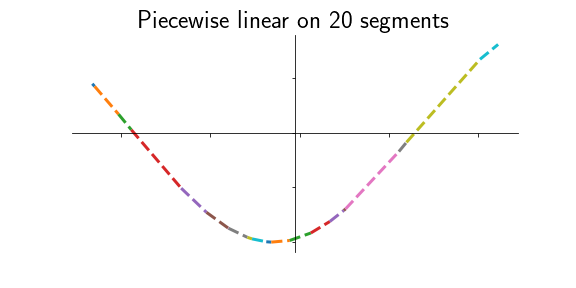
\includegraphics[width=0.5\textwidth]{pl_2.png}
  \underline{Result}: $\exists! f \in \$_{2, {\bf t}}$ such that $f(t_i) = g(t_i)$
  \mbox{}\\
  \mbox{}\\
  \mbox{}\\
  \mbox{}\\
  \mbox{}\\
  \mbox{}\\
}

\frame{\frametitle{Interpolator $I_2$}
  \underline{Not.}
  \begin{itemize}
    \itemsep0em
    \item $a=t_1 < \cdots < t_n=b$,  $g: [a,b] \to \mathbb{R}$
    \item $\Pi_{<n, {\bf t}} = \{\text{pp of order $n$ with breaks at $t_2, \ldots, t_{n-1}$}\}$
    \item $\$_{2, {\bf t}} = \Pi_{<2, {\bf t}} \cap \mathcal{C}^0$
  \end{itemize}
  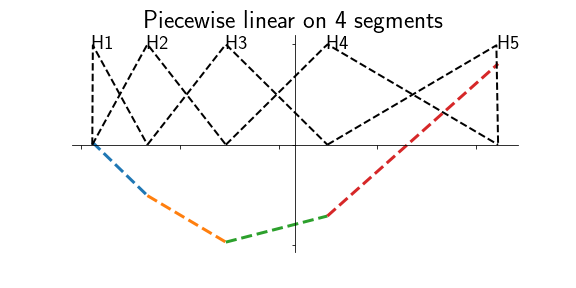
\includegraphics[width=0.5\textwidth]{pl_1_hat.png}%
  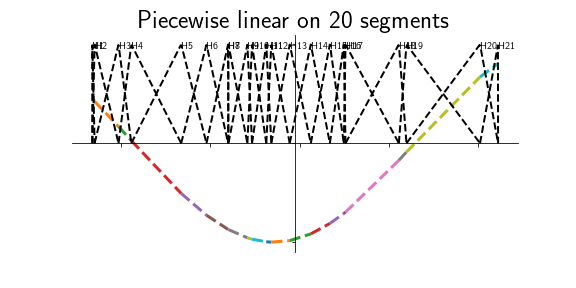
\includegraphics[width=0.5\textwidth]{pl_2_hat.png}
  \underline{Result}: $\exists! f \in \$_{2, {\bf t}}$ such that $f(t_i) = g(t_i)$
  \begin{equation}
    \phi_i(t) = \begin{dcases}
      \frac{t-t_{i-1}}{t_i-t_{i-1}} & \text{if} \ t_{i-1} < t \leq t_i \\
      \frac{t_{i+1}-t}{t_{i+1}-t_{i}} & \text{if} \ t_i \leq t < t_{i+1}
    \end{dcases}
    ,\qquad
    I_2g = \sum_{i=1}^n g(t_i)\phi_i
  \end{equation}
}

%%%%%%%%%%%%%%%
%% FRAME 9 
%%%%%%%%%%%%%%%

\frame{\frametitle{Approximation power of $I_2$}
 \underline{Not.}
  \begin{itemize}
    \itemsep0em
    \item $a=t_1 < \cdots < t_n=b$, $g: [a,b] \to \mathbb{R}$
    \item $I_2g = \sum_{i=1}^n g(t_i)\phi_i \in \$_{2, {\bf t}}$
  \end{itemize}
  \underline{Properties}
  \begin{prop}{4}
  \begin{enumerate}
    \item For $f \in \$_{2, {\bf t}}, I_2f=f$
    \item $\|I_2g\| \leq \|g\|$
      \pause%
    \item If $g \in \mathcal{C}^{(2)}$, $\|g-I_2g\| \leq \frac{|{\bf t}|^2}{8} \|g''\|$
    \item If $g \in \mathcal{C}^0$, $\|g-I_2g\| \leq w(g, |{\bf t}|)$.
  \end{enumerate}
  \end{prop}
}

\subsection{II/2 Piecewise cubic interpolation}

\frame{\frametitle{Cubic pieces}
 \underline{Not.}
  \begin{itemize}
    \itemsep0em
    \item $a=t_1 < \cdots < t_n=b$, $g: [a,b] \to \mathbb{R}$
    \item $g(t_1), s_1, \dots, g(t_n), s_n$
  \end{itemize}
  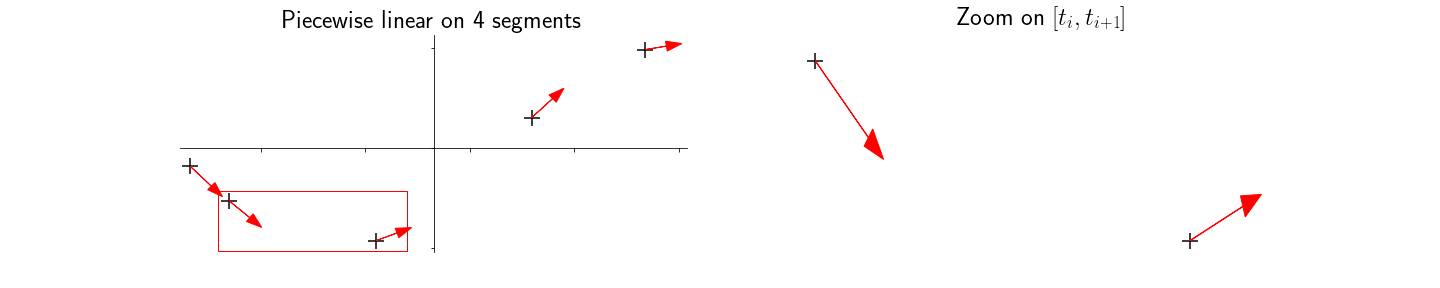
\includegraphics[width=\textwidth]{pc_1.png}
  \pause%
  On $[t_i, t_{i+1}]$, 4 conditions for $f_{|[t_i, t_{i+1}]}$ $\implies \exists! f_i \in \Pi_{<4}$ s.t $f_i=f_{|[t_i, 
  t_{i+1}]}$
  \pause%
  (Newton form)
  \begin{small}
  \begin{align*}
    f_{|[t_i, t_{i+1}]} &= [t_i]f_i + (t-t_i)[t_i, t_i]f_i + {(t-t_i)}^2[t_i, t_i, t_{i+1}]f_i \\
    & + {(t-t_i)}^2(t-t_{i+1})[t_i, t_i, t_{i+1}, t_{i+1}]f_i
   \end{align*}
 \end{small}
}

\frame{\frametitle{Explicit formula}
  \begin{small}
    \begin{align*}
      f_{|[t_i, t_{i+1}]}(t) &= g(t_i) + s_i {(t-t_i)}^2+ (3\frac{\Delta g(t_i)}{\Delta t_i^2} - \frac{s_i + 
      s_{i+1}}{\Delta t_i}){(t-t_i)}^3 \\
    &+ (\frac{s_i + s_{i+1}}{\Delta t_i^2} - 2\frac{\Delta g(t_i)}{\Delta t_i^3}){(t-t_i)}^4 
  \end{align*}
 \end{small}
}

\frame{\frametitle{4 cases}
  \setlength{\abovedisplayskip}{-1pt}
  \setlength{\belowdisplayskip}{-4pt}
  \begin{itemize}
    \item \underline{case 1} $(s_i) = (g'(t_i))$ i.e \textbf{Hermite} interp\@.
      \begin{equation*}
        \text{if} \quad g \in \mathcal{C}^{(4)}, \|g-f\| \leq \frac{1}{384} |{\bf t}|^4 \|g^{(4)}\| \quad  \text{De Boor 
        1978}
      \end{equation*}
      \pause%
    \item \underline{case 2} Enforce $f \in \mathcal{C}^{(2)}$ i.e $f''_{|[t_{i-1}, t_i]}(t_i) = f''_{|[t_{i}, 
      t_{i+1}]}(t_i) \implies$  tridiagonal linear system for $s_2, \ldots, s_{n-1}$.\\
      \pause%
      \begin{itemize}
        \item \underline{case 2a}
          $s_1 = g'(t_1), s_n = g'(t_n)$ \textbf{Complete} cubic spline.  
          \begin{equation*}
          \|g-f\| = \mathcal{O}(|t|^4) \quad  \text{De Boor 1978}
         \end{equation*}
          \pause%
        \item \underline{case 2b}
          $s_1, s_n$ unknown, enforce $f''(t_1) = f''(t_n) = 0$ \textbf{Natural} cubic spline
          \begin{equation*}
            \|g-f\| = \mathcal{O}(|t|^2) \quad  \text{De Boor 1978}
          \end{equation*}
          \pause%
        \item \underline{case 2c}
          $s_1, s_n$ unknown, enforce continuity of $f^{(3)}$ at $t_2$ and $t_n$ \textbf{Not-a-knot} condition.
          \begin{equation*}
              \|g-f\| = \mathcal{O}(|t|^4) \quad \text{Schwartz \& Vozga 1972}
            \end{equation*}
      \end{itemize}
  \end{itemize}
}

\frame{\frametitle{Examples}
  \begin{enumerate}
    \item $(s_i) = (g'(t_i))$. Cubic Hermite interpolation.
      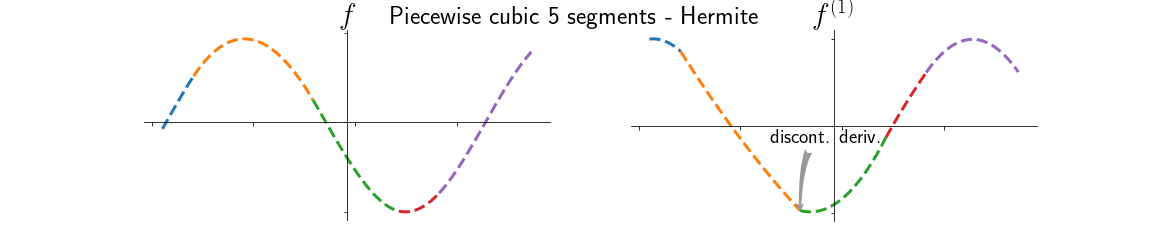
\includegraphics[width=\linewidth]{cubic_1.png}
      \pause%
    \item $n-2$ equations $ f''(t_i) = f''(t_{i+1})$. Cubic spline interpolation.
      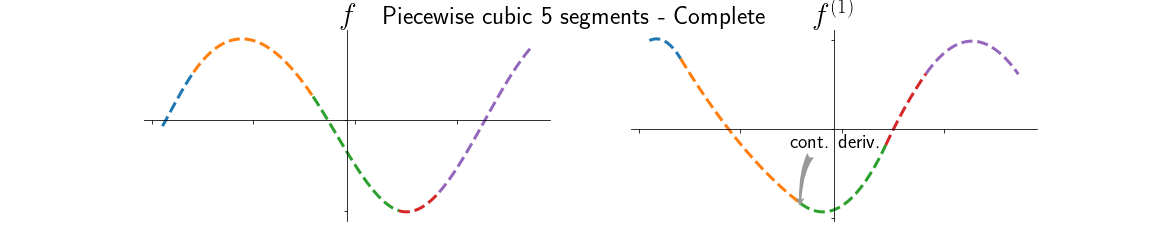
\includegraphics[width=\linewidth]{cubic_2.png}
  \end{enumerate}
}

\frame{\tableofcontents}

\section{III/ B-splines and Splines}

\subsection{III/1 Definition and fundamental properties}

\frame{\frametitle{Formal definition B-splines}
     \underline{Not.}
      \begin{itemize}
        \itemsep0em
        \item $\cdots \leq t_i \leq t_{i+1} \leq \cdots $ finite or infinite
      \end{itemize}
      \pause%
    Two different normalizations
    \begin{deftn}{2  C. De Boor 1978}
      The $j^{th}$ (normalized B-spline) of order $k$ is
      \begin{equation}
        B_{j, k, \bm{t}}(t) = (t_{j+k}-t_j)[t_j, \ldots, t_{j+k}]{(.-t)}_+^{k-1}
      \end{equation}
    \end{deftn}
    \pause%
    \begin{deftn}{3 Schoenberg 1973}
      The $j^{th}$ B-spline of order $k$ is given by
      \begin{equation}
        M_{j, k, \bm{t}}(t) = \frac{1}{k} [t_j, \ldots, t_{j+k}]{(.-t)}_+^{k-1}
      \end{equation}
    \end{deftn}
}

\frame{\frametitle{First properties}
  \begin{prop}{5}
    \begin{enumerate}
      \item (pp function) $B_{j, k, \bm{t}} \in \Pi_{<k, \bm{t}}$
      \item (rec\@. relation)  \begin{equation*}
        B_{j, k} = w_{j,k} B_{j, k-1} + (1-w_{j+1,k}) B_{j+1, k-1} \qquad w_{jk}(t) = \frac{t-t_{j}}{t_{j+k}-t_j}
      \end{equation*}
    \item (supp\@. and pos) \begin{itemize}
        \itemsep0em
        \item $B_{j,k} = 0$ outside $[t_j, t_{j+k}]$
        \item $B_{j, k} > 0$ on $(t_j, t_{j+k})$
        \end{itemize}
    \end{enumerate}
  \end{prop}
  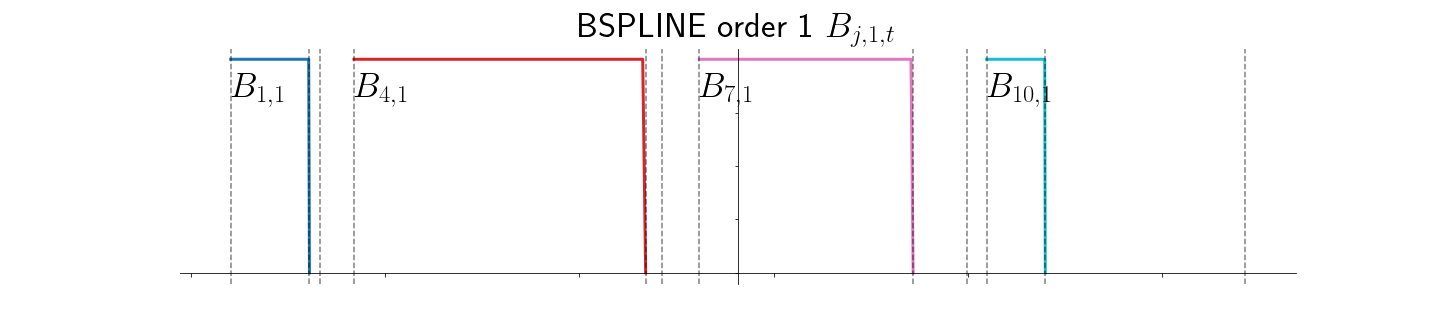
\includegraphics[width=\linewidth]{bspline_order_1.png}
}

\frame{\frametitle{First properties}
  \begin{prop}{5}
    \begin{enumerate}
      \item (pp function) $B_{j, k, \bm{t}} \in \Pi_{<k, \bm{t}}$
      \item (rec\@. relation)  \begin{equation*}
        B_{j, k} = w_{j,k} B_{j, k-1} + (1-w_{j+1,k}) B_{j+1, k-1} \qquad w_{jk}(t) = \frac{t-t_{j}}{t_{j+k}-t_j}
      \end{equation*}
    \item (supp\@. and pos) \begin{itemize}
        \itemsep0em
        \item $B_{j,k} = 0$ outside $[t_j, t_{j+k}]$
        \item $B_{j, k} > 0$ on $(t_j, t_{j+k})$
        \end{itemize}
    \end{enumerate}
  \end{prop}
  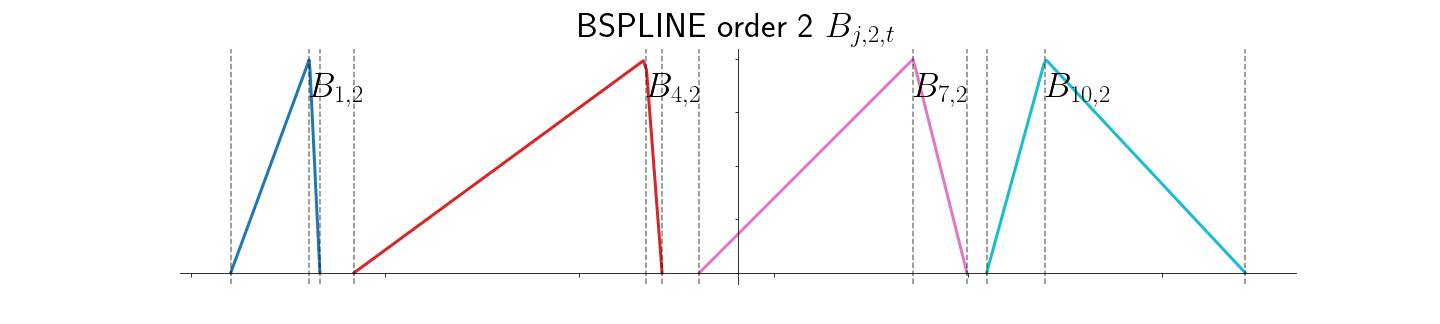
\includegraphics[width=\linewidth]{bspline_order_2.png}
}

\frame{\frametitle{First properties}
  \begin{prop}{5}
    \begin{enumerate}
      \item (pp function) $B_{j, k, \bm{t}} \in \Pi_{<k, \bm{t}}$
      \item (rec\@. relation)  \begin{equation*}
        B_{j, k} = w_{j,k} B_{j, k-1} + (1-w_{j+1,k}) B_{j+1, k-1} \qquad w_{jk}(t) = \frac{t-t_{j}}{t_{j+k}-t_j}
      \end{equation*}
    \item (supp\@. and pos) \begin{itemize}
        \itemsep0em
        \item $B_{j,k} = 0$ outside $[t_j, t_{j+k}]$
        \item $B_{j, k} > 0$ on $(t_j, t_{j+k})$
        \end{itemize}
    \end{enumerate}
  \end{prop}
  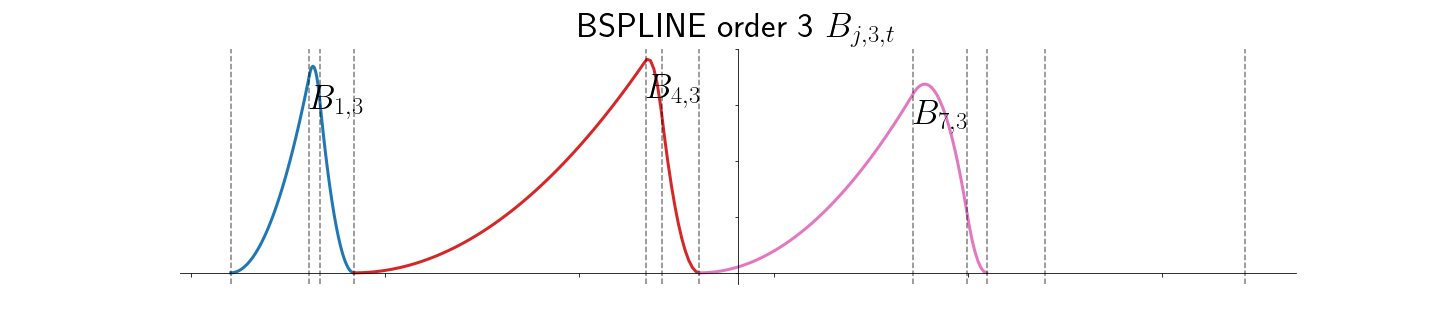
\includegraphics[width=\linewidth]{bspline_order_3.png}
}

\frame{\frametitle{First properties}
  \begin{prop}{5}
    \begin{enumerate}
      \item (pp function) $B_{j, k, \bm{t}} \in \Pi_{<k, \bm{t}}$
      \item (rec\@. relation)  \begin{equation*}
        B_{j, k} = w_{j,k} B_{j, k-1} + (1-w_{j+1,k}) B_{j+1, k-1} \qquad w_{jk}(t) = \frac{t-t_{j}}{t_{j+k}-t_j}
      \end{equation*}
    \item (supp\@. and pos) \begin{itemize}
        \itemsep0em
        \item $B_{j,k} = 0$ outside $[t_j, t_{j+k}]$
        \item $B_{j, k} > 0$ on $(t_j, t_{j+k})$
        \end{itemize}
    \end{enumerate}
  \end{prop}
  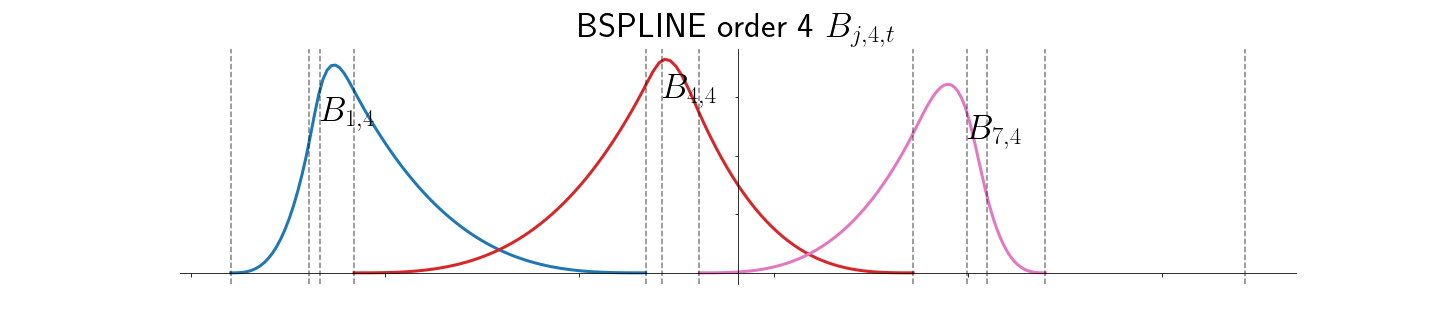
\includegraphics[width=\linewidth]{bspline_order_4.png}
}

\frame{\frametitle{More properties}
  \begin{deftn}{4}
    A spline is a linear combination of B-splines.
    \begin{equation*}
      \$_{k, {\bm t}} = \{ \sum_{j} c_j B_{j,k} | c_j \ \text{real}\}
    \end{equation*}
  \end{deftn}
  \pause%
  \begin{enumerate}
    \item (partition unity) $\displaystyle \sum_{j \in \mathbb{Z}} B_{j,k} = 1$
    \item (Riesz-basis norm sup) $\exists D_{k} \in (0,1)$ such that $\forall \bm{c}$ bounded,
      \begin{equation*}
        D_{k} \|\bm{c}\| \leq \|\sum_{j} c_j B_{j,k} \| \leq  \|\bm{c}\| \quad \text{De Boor 1976}
      \end{equation*}
    \item (Marsden's identity) For any $\tau \in \mathbb{R}$,
      \begin{equation*}
        {(.-\tau)}^{k-1} = \sum_{j} \psi_{j,k}(\tau) B_{j,k} \quad \psi_{j,k}(\tau) = (t_j - \tau)\cdots(t_{j+k-1}-\tau)
      \end{equation*}
  \end{enumerate}
}

\frame{\frametitle{Multiple knots}
  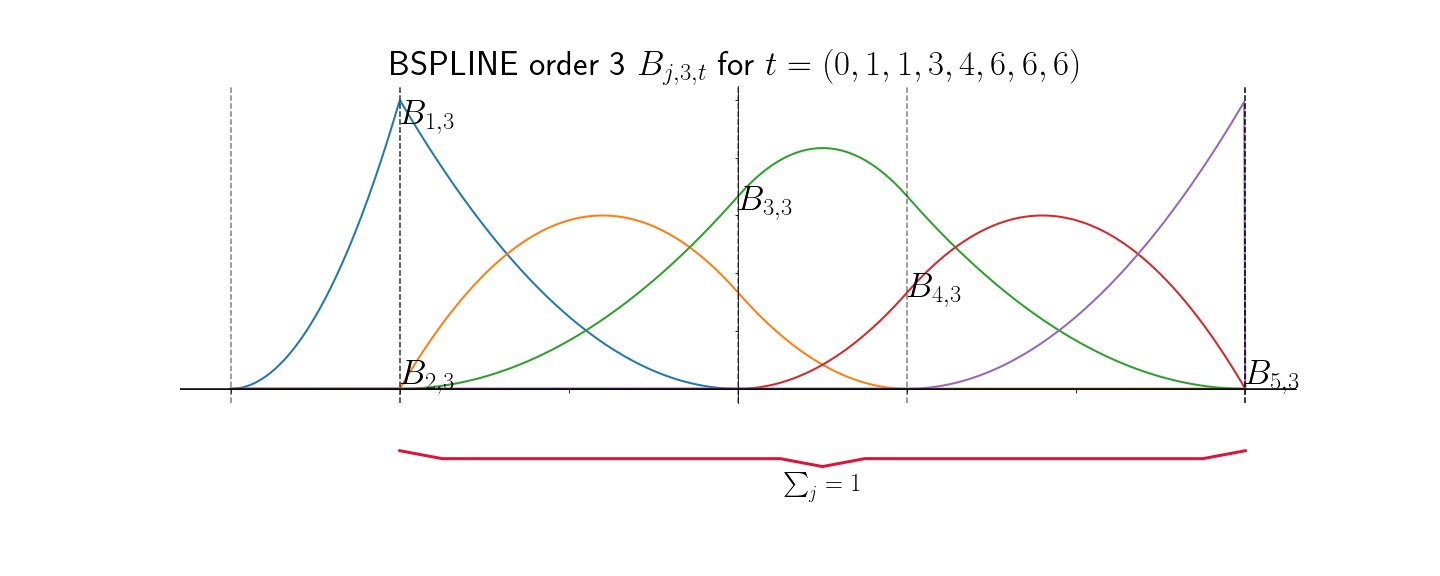
\includegraphics[width=\linewidth]{bspline_mult.png}
}


\subsection{III/2 Applications}

\frame{\frametitle{Applications}
  \begin{enumerate}
    \item In practice, choose ${\bm t} = \mathbb{Z}_r$ with $r \geq 1$.
      \begin{itemize}
        \item Landmark paper by Schoenberg \underline{Contributions to the problem of approximation of equidistant} 
          \underline{data by analytic functions: part A}, \emph{Quarterly of Applied Mathematics}. Vol 4 pp 45-99.  1946
          \pause%
        \item M. Unser \underline{Splines: A perfect fit for signal and image processing}, IEEE\@. Vol 16 pp 22-38 
          1999.\\
          \begin{equation}
            B_{0,1} = \beta_+^{0}, \quad B_{j,n} = \beta_+^{n}(-.j) \underbrace{\beta_+^{0}*\dots*\beta_+^{0}}_{(n-1) 
            \text{times}}(.-j)
          \end{equation}
          \begin{equation}
            \sum_{j \in \mathbb{Z}} c[j] \beta^n(.-j) \quad \beta^n = \beta_+(.+\frac{n+1}{2})
          \end{equation}
      Allows for efficient algorithms and Fourier analysis,
      \begin{equation*}
        \hat{\beta}_+^n(w) = {\left(\frac{1-e^{-jw}}{jw}\right)}^n
      \end{equation*}
      \end{itemize}
  \end{enumerate}
}

\frame{\frametitle{Applications}
  \begin{enumerate}
    \item In practice, choose ${\bm t} = \mathbb{Z}_r$ with $r \geq 1$.
    \item Critical choice of \textbf{generators} ${(\phi_j)}_{j \in \mathbb{Z}}$
      \begin{enumerate}
        \setlength{\abovedisplayskip}{-1pt}
        \setlength{\belowdisplayskip}{-4pt}
        \item Delgado et al. \underline{Snakes with an ellipse-reproducing property}, \emph{IEEE\@}. Vol 21, 2012.
          \begin{equation*}
            r = \sum_{j} \begin{bmatrix} c_1[j] \\ c_2[j] \end{bmatrix} \phi_j \quad \text{with} \ \phi_j = \phi(.-j) 
            \quad \text{with} \quad \phi(t) = \lambda_0 \beta_{\alpha}(t+\frac{3}{2})
          \end{equation*}
          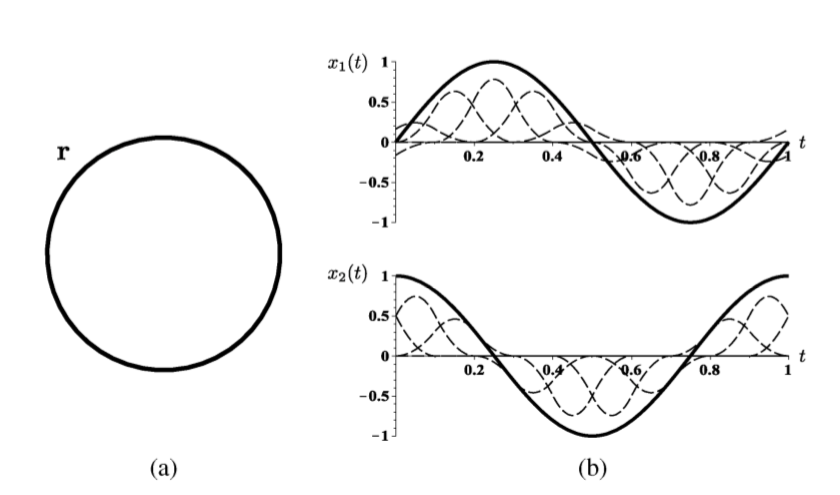
\includegraphics[width=0.8\linewidth]{delgado_2012.png}
      \end{enumerate}
  \end{enumerate}
}

\frame{\frametitle{Applications}
  \begin{enumerate}
    \item In practice, choose ${\bm t} = \mathbb{Z}_r$ with $r \geq 1$.
    \item Critical choice of \textbf{generators} ${(\phi_j)}_{j \in \mathbb{Z}}$
      \begin{enumerate}
        \setlength{\abovedisplayskip}{-1pt}
        \setlength{\belowdisplayskip}{-4pt}
        \item Delgado et al. \underline{Snakes with an ellipse-reproducing property}, \emph{IEEE\@}. Vol 21, 2012.
        \item Uhlmann et al. \underline{Hermite snakes with control of tangents}, \emph{IEEE\@}. Vol 25, 2016.
          \begin{equation*}
            r = \sum_{j} \begin{bmatrix} c^1_1[j] \\ c^1_2[j] \end{bmatrix} \phi^1_j + \begin{bmatrix} c^2_1[j] \\ 
          c^2_2[j] \end{bmatrix} \phi^2_j \quad \text{with} \ \phi^1_j, \phi^2_j \in \$_{4, \mathbb{Z}_2}            
        \end{equation*}
          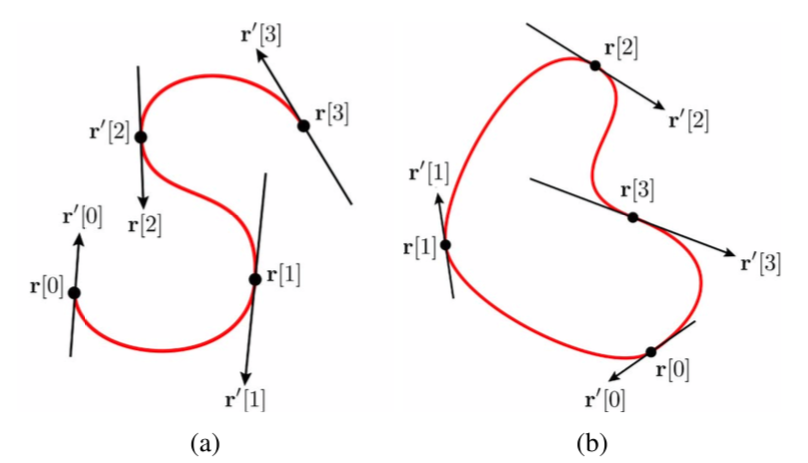
\includegraphics[width=0.7\linewidth]{uhlmann_2016.png}
      \end{enumerate}
  \end{enumerate}
}


\frame{\frametitle{Applications}
  \begin{enumerate}
    \item In practice, choose ${\bm t} = \mathbb{Z}_r$ with $r \geq 1$.
    \item Critical choice of \textbf{generators} ${(\phi_j)}_{j \in \mathbb{Z}}$
    \item Things to consider
      \begin{itemize}
        \item Space of reproducible functions
          \begin{equation*}
            V = \text{span}{(\phi_j)} \cap L_2 = \{\sum_{j \in \mathbb{Z}} c[j] \phi_j | c[j] \in \mathbb{R} \} \cap L_2
            \end{equation*}
          \pause%
          \item Desired properties in CAGD
            \begin{enumerate}
              \item Affine invariance i.e $s \in V \implies As + b \in V$. True if $\sum_j \phi_j = 1$
              \item Unicity and stability. True if $(\phi_j)$ is a Riesz-basis in $L_2$ i.e $\exists 0 < m, M$
                \begin{equation*}
                  m {\|c\|}_{l_2}^2 \leq {\left\|\sum_{j}  c[j] \phi_j \right\|}_{L_2}^2 \leq  M{\|c\|}_{l_2}^2
              \end{equation*}
            \end{enumerate}
         \pause%
       \item Reproducible functions
         \begin{enumerate}
           \item Polynomial, exponential polynomials
           \item Smoothness
         \end{enumerate}
       \pause%
       \item Approximation power as number of control points increases
    \end{itemize}
  \end{enumerate}
}

%\section{II/ Introduction to spline curves}
%\subsection{II/1 Cardinal B-splines}
%%
%%
%%\frame{\frametitle{Kesako?}
%%  \begin{enumerate}
%%    \item[3] $\sum_j B_{j, k, \bm{t}} = 1$ on $[t_k, t_{n+1}]$ (if $\bm{t} = {(t_i)}_{1}^{n+k}$)
%%    \item[4] In neighborhood of $t_j$ $B_{j,k,t}$ is $\mathcal{C}^{k-1-r}$ with $r$ multiplicity of $t_j$
%%  \end{enumerate}
%%%  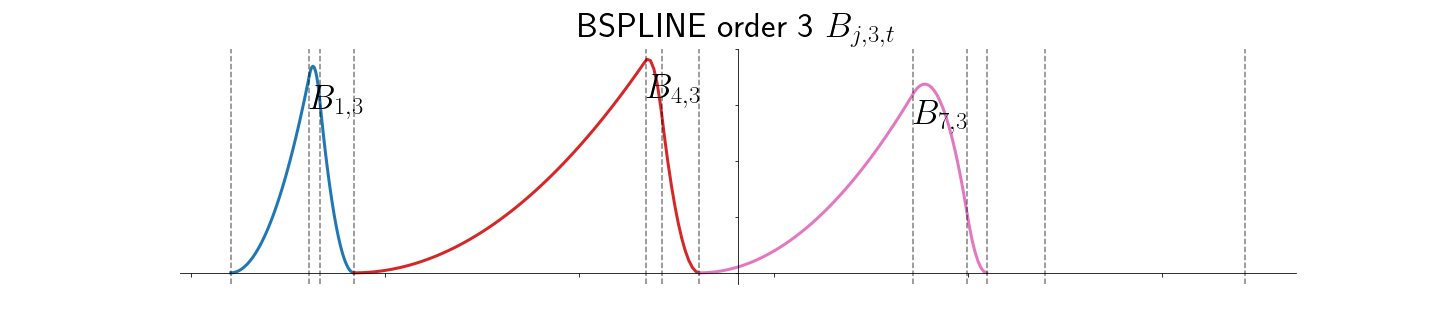
\includegraphics[width=\linewidth]{bspline_order_3.png}
%%  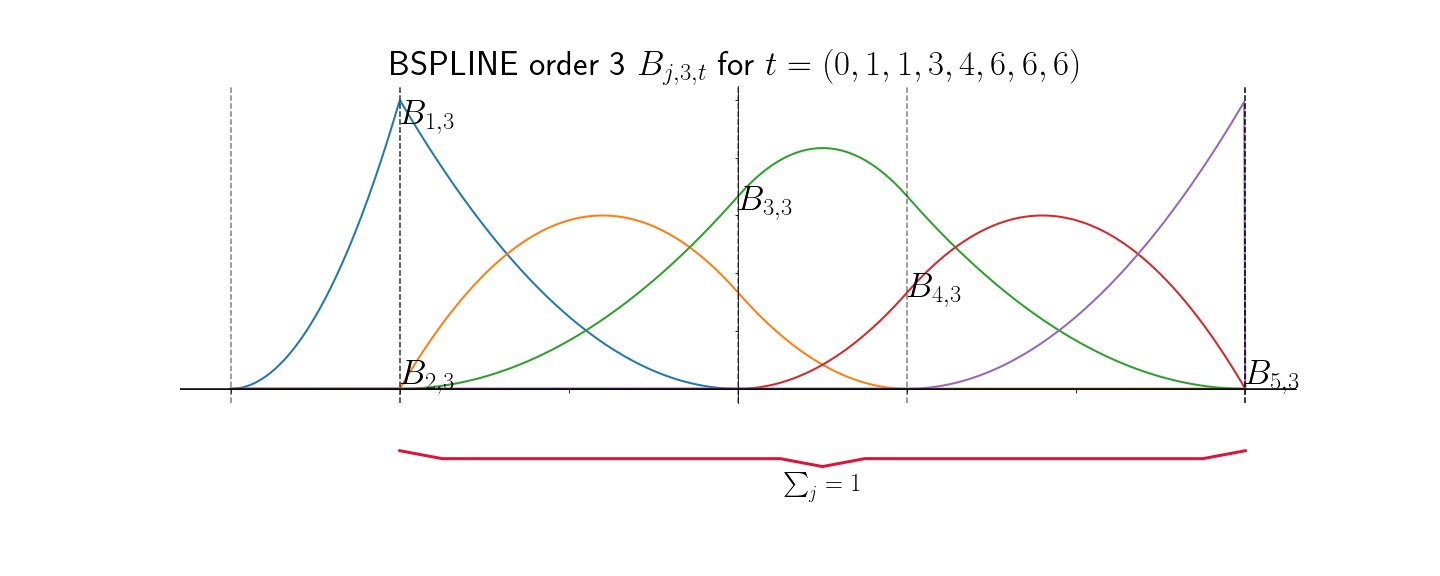
\includegraphics[width=\linewidth]{bspline_mult.png}
%%  Example: knot $t_2=t_3=1$ has multiplicity 2. 
%%}
%
%\frame{\frametitle{The B-spline basis}
%  \begin{deftn}{1}
%    \begin{small}
%    The cardinal B-spline of order $n$ (and knot multiplicity 1) is given by recursive relation
%    \begin{equation}
%      B^n = B^1 * B^1 * \ldots * B^1 \quad (\text{n times})
%    \end{equation}
%      with $B^1(t) = \begin{dcases}
%          1 &\text{if } 0 \leq 1 < 1 \\
%          0 &\text{else } \\
%        \end{dcases}$
%    \end{small}
%  \end{deftn}
%  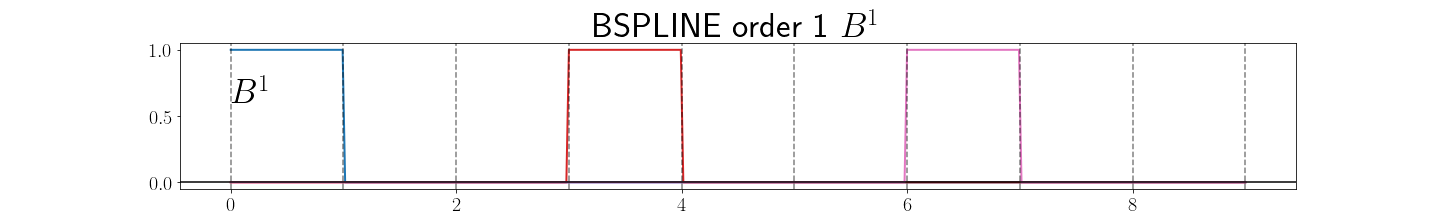
\includegraphics[width=\linewidth]{card_order_1.png}
%  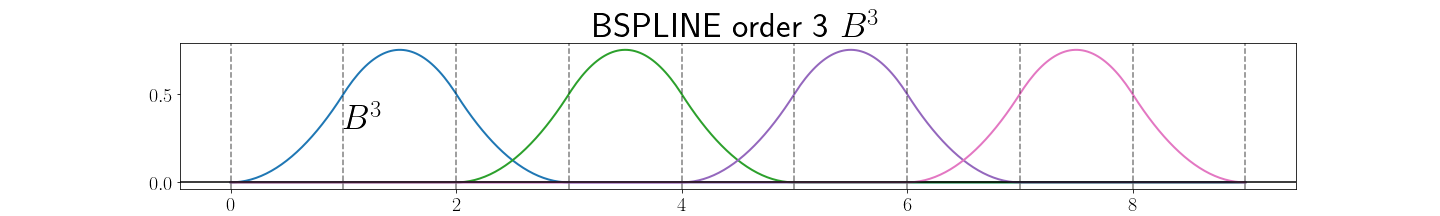
\includegraphics[width=\linewidth]{card_order_3.png}
%}
%
%
%\frame{\frametitle{Spline curve}
%  \begin{deftn}{1}
%    \begin{small}
%    A (cardinal) \textbf{spline} or order $n$ (and knot multiplicity 1) is a linear combination of $\{B^n(.-k)\}$
%    \begin{equation}
%      f(t) = \sum_{k \in \mathbb{Z}} c[k] B^n(t-k)
%    \end{equation}
%    with $c[k] \in \mathbb{R}$. We denote $S_{n,1}$ the set of all such functions.
%  \end{small}
%  \end{deftn}
%  \pause%
%  \underline{Remarks}
%  \begin{enumerate}
%    \item $(c[k])$ is the sequence of \textbf{control points}.
%    \item $S_{n,1} \subset \Pi_{<n, \mathbb{Z}} \cap \mathcal{C}^{n-2}$ (in fact these sets are equal!)
%    \item $r_k = \#\{l| t_l = k\}$ (multiplicity), $f$ is $\mathcal{C}^{n-r_k-1}$ in $\mathcal{V}(k)$.
%    \item Denote $S_{n,r}$ splines of order $n$ with knots of multiplicity $r$.
%    \item A \textbf{spline curve} is a vector-valued spline i.e $c[k] \in \mathbb{R}^d$ (d=2,3 usually)
%  \end{enumerate}
%}
%
%\frame{\frametitle{Dream pursued}
%  Find approximation scheme $f$ interpolating $(\bm{y}_k)$
%  \begin{equation}
%  f(t) = \sum_{k} \bm{y}_k^T \bm{\phi}(t-t_k) \end{equation}
%  and $\bm{\phi}$ retains good properties of splines (partition-unity, Riesz-basis, compact support, subdivision).
%}
%
%\subsection{II/2 Schoenberg theorems}
%\frame{\frametitle{Hermite interpolation}
%  Let $\mathcal{S}$ a vector space.  C.H.I.P ($y$, \ldots, $y^{(r-1)}$, $\mathcal{S}$) is solved if $\exists f \in 
%  \mathcal{S}$ such that
%  \begin{equation}
%    \forall s=0, \ldots, r-1, \forall k \in \mathbb{Z} \qquad f^{(s)}(k) = y^{(s)}_k
%  \end{equation}
%    \pause%
%    \begin{thm}{1}
%    \begin{small}
%      $n$ even, $1 \leq r \leq n/2$. The C.H.I.P ($y$, \ldots, $y^{(r-1)}$, $S_{n,r} \cap F_{\gamma, r}$ (resp.  
%      $\mathcal{L}_{p,r}$)) has a unique solution iif $y^{(s)} \in Y_{\gamma}$ (resp. $l_p$). \underline{In that case}
%    \begin{equation}
%      f(t) = \sum_{k \in \mathbb{Z}} y_k L_{n,r,0}(t-k) + \ldots, y^{(r-1)}_k L_{n,r-1}(t-k)
%    \end{equation}
%  \end{small}
% \end{thm}
% \underline{Remarks}
% \begin{enumerate}
%   \item $L_{n,r,s}$ are elements of $S_{n,r}$. Calculated by solving system of $n-r$ equations.
%   \item $f \in S_{n,r}$ is a \textbf{spline} of order $n$
% \end{enumerate}
%}
%
%\frame{\frametitle{Hermite snakes (Uhlmann 2016)}
%  \underline{Data}: at $M$ sites ${\{r[k]\}}_{k=0}^{M-1},{\{r'[k]\}}_{k=0}^{M-1}$. \\
%  \underline{Obj}: Continuous representation of the curve $r(t) = (r_1(t), r_2(t))$ \\
%  \pause%
%  \smallbreak%
%  Schoenberg for $n=4$ and $r=2$\\
%  \begin{equation}
%    r(t) = \sum_{k \in \mathbb{Z}} r[k] \phi_1(t-k) + r'[k] \phi_2(t-k)
%  \end{equation}
%    
%  $\phi_1 = L_{4, 2, 0}, \phi_2 = L_{4,2,1}$ (polynomials order 4). $r_1, r_2 \in \mathcal{C}^{n-r-1} = \mathcal{C}^1$.
%  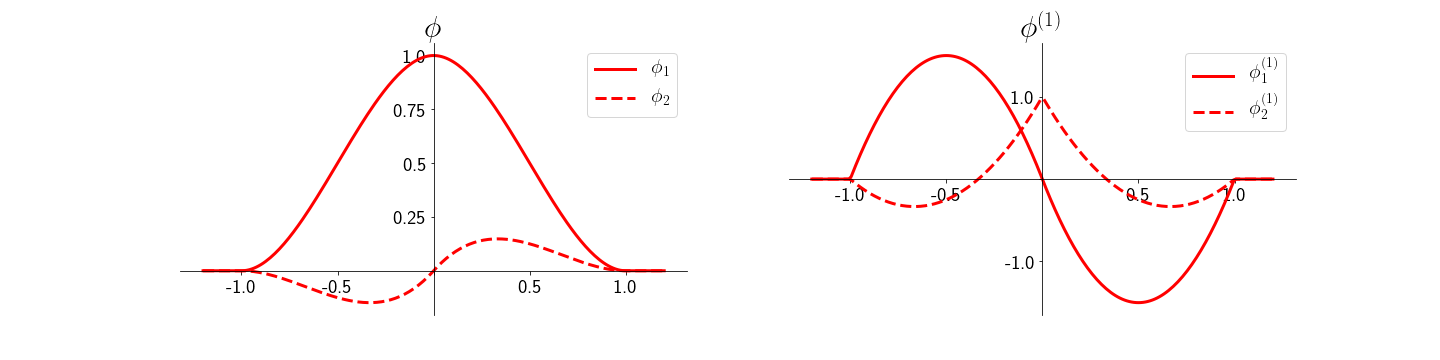
\includegraphics[width=\linewidth]{hermite_uhl.png}
%}
%
%\frame{\frametitle{Hermite snakes (Uhlmann 2016)}
%  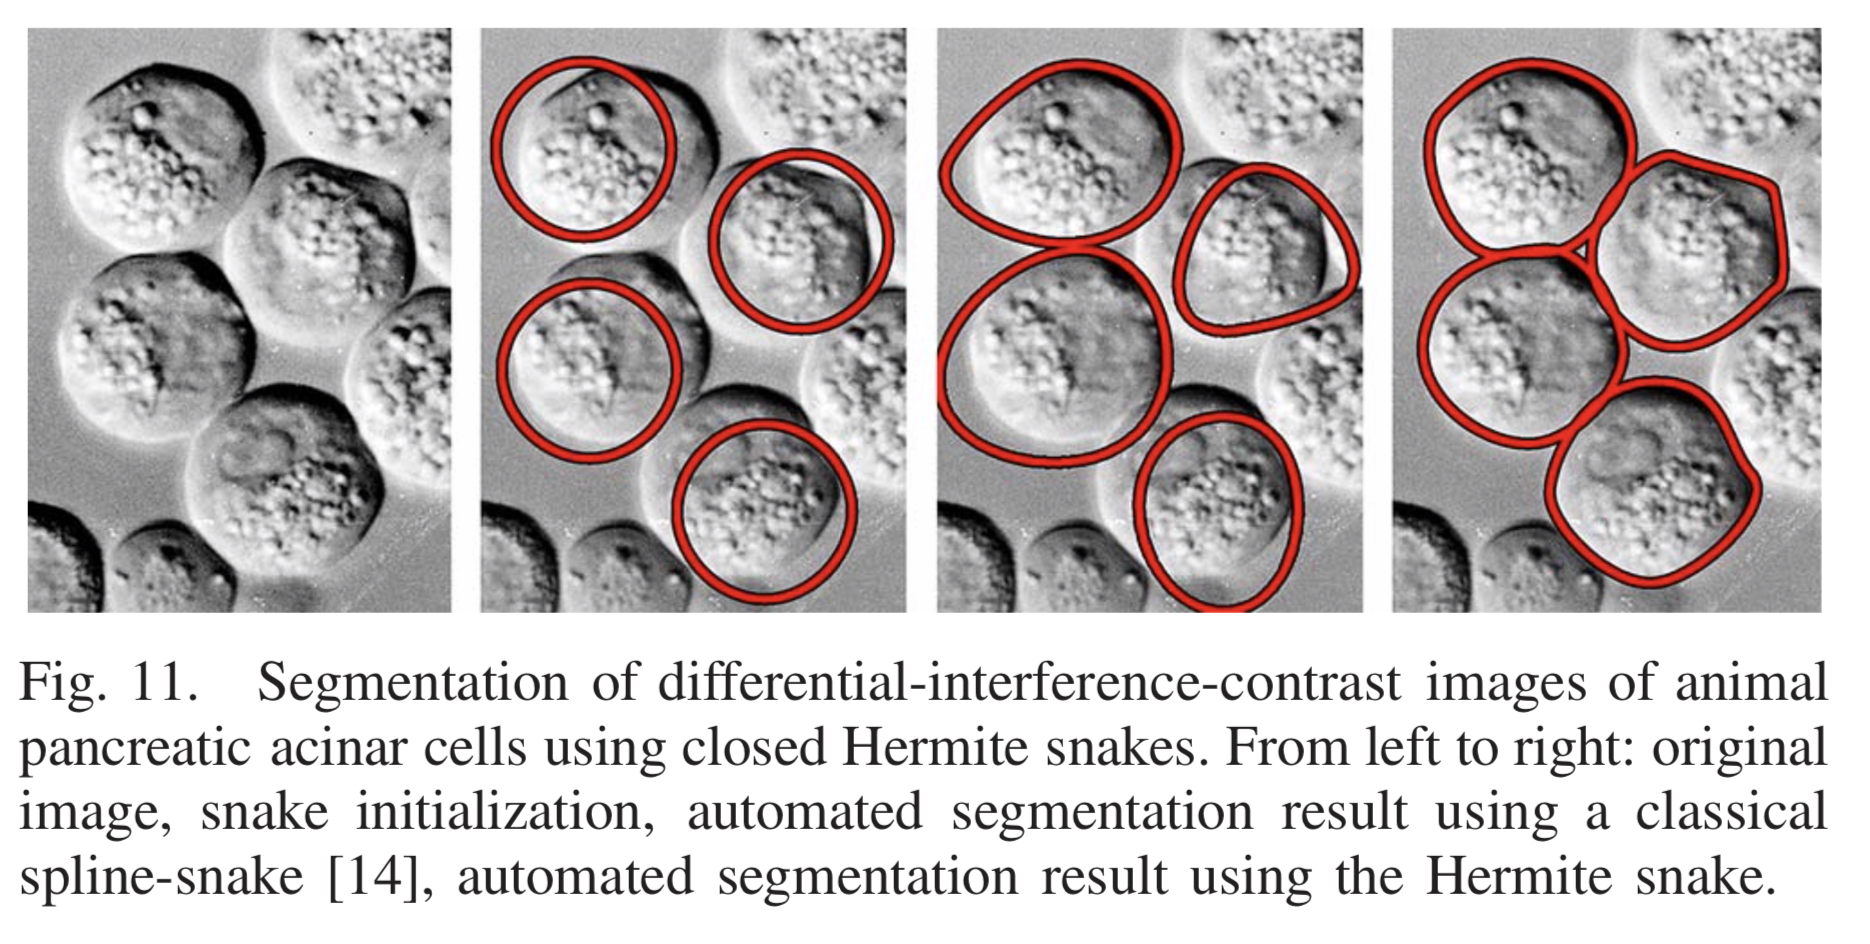
\includegraphics[width=\linewidth]{hermite_ex.png}
%}
%
%\subsection{II/3 Ellipse-preserving snakes}
%\frame{\frametitle{Ellipse-preserving Hermite (Conti 2015)}
%  \underline{Data}: at $M$ sites ${\{r[k]\}}_{k=0}^{M-1},{\{r'[k]\}}_{k=0}^{M-1}$. \\
%  \underline{Obj}: Continuous representation of the curve $r(t) = (r_1(t), r_2(t))$. Good basis and \textbf{reproduction 
%  of unit circle.}
%  \pause%
%  \begin{equation}
%    \quad r(t) = \sum_{k \in \mathbb{Z}} r[k] \phi_1(t-k) + r'[k] \phi_2(t-k)
%  \end{equation}
%  
%  with $\phi_i(t) = \left(a_i(t) + b_i(t)t + c_i(t) e^{jwx} + d_i(t) e^{-jwx}\right) \chi_{[-1,1]}$ and $w = 
%  \frac{2\pi}{M}$ (exponential polynomials).\\
%  \medbreak%
%  \underline{Remark}: here the curve is said to be an \textbf{exponential spline curve}
%}
%
%\frame{\frametitle{Ellipse-preserving Hermite (Conti 2015)}
%  Reproducing sinusoids with $M$ coefficients
%  \begin{align}
%    \cos (2\pi t) &= \sum_{k \in \mathbb{Z}} \cos (\frac{2\pi k}{M}) \phi_1(Mt-k) - \frac{2\pi}{M} \sin (\frac{2\pi 
%    k}{M}) \phi_2(Mt-k) \\
%  \sin (2\pi t) &= \sum_{k \in \mathbb{Z}} \sin (\frac{2\pi k}{M}) \phi_1(Mt-k) + \frac{2\pi k}{M} \cos (\frac{2\pi 
%  k}{M}) \phi_2(Mt-k)
%  \end{align}
%  }
%
%\frame{\tableofcontents}
%
%\section{III/ Representation of spline surfaces}
%\subsection{III/1 Extension of Conti's scheme}
%\frame{\frametitle{The case of the unit sphere}
%  The sphere surface parametrized by $g=\sigma: \mathbb{R}^2 \to \mathbb{R}^3$
%  \begin{equation}
%    \sigma(u,v) = \begin{bmatrix} \cos(2\pi u)\sin(\pi v) \\ \sin(2\pi u)\sin(\pi v) \\ \cos(\pi v) \end{bmatrix} \quad 
%    (u, v) \in {[0,1]}^2
%  \end{equation}
%  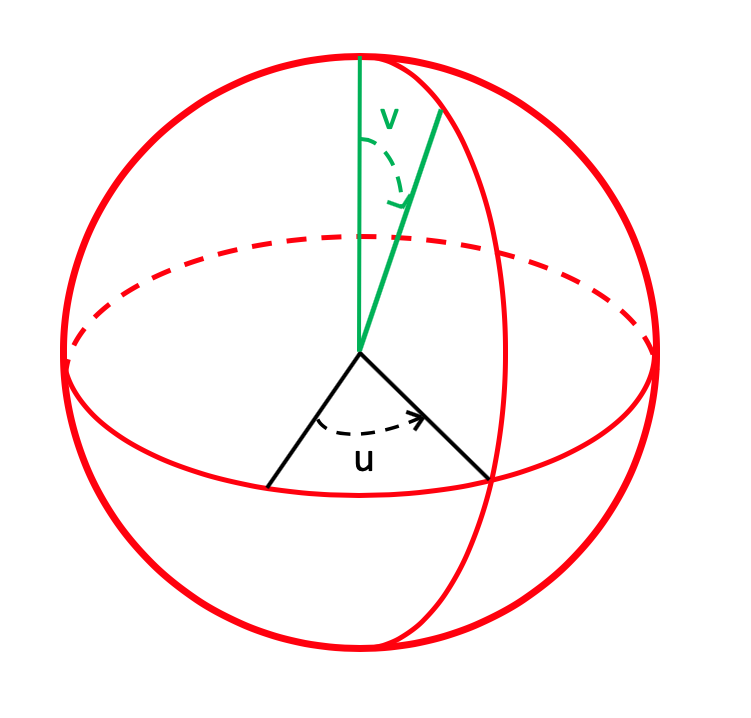
\includegraphics[width=0.4\linewidth]{sphere_param.png}
%}
%
%\frame{\frametitle{From 2D to 3D for tensor-product surfaces}
%  \underline{Data}: $M_1$ control points on latitudes, $M_2+1$ control points on longitudes. At each point $4$ 
%  parameters $\sigma, \partial^{1,0} \sigma, \partial^{0,1} \sigma, \partial^{1,1} \sigma$. \\
%  \underline{Obj}: Continuous representation of $g:\mathbb{R}^2 \to \mathbb{R}^3$ \\
%  \pause%
%    \begin{align*}
%      \sigma(u,v) &= \sum_{k=0}^{M_1-1} \sum_{l=0}^{M_2} c_1[k,l]\phi_{1, w_1, per}(M_1u-k)\phi_{1, w_2}(M_2v-l) \\
%      &+ \sum_{k=0}^{M_1-1} \sum_{l=0}^{M_2} c_2[k,l] \phi_{1, w_1, per}(M_1u-k)\phi_{2, w_2}(M_2v-l) \\
%      &+ \sum_{k=0}^{M_1-1} \sum_{l=0}^{M_2} c_3[k,l] \phi_{2, w_1, per}(M_1u-k)\phi_{1, w_2}(M_2v-l) \\
%      &+ \sum_{k=0}^{M_1-1} \sum_{l=0}^{M_2} c_4[k,l] \phi_{2, w_1, per}(M_1u-k)\phi_{2, w_2}(M_2v-l) \\
%    \end{align*}
%  }
%
%\frame{\frametitle{From 2D to 3D for tensor-product surfaces}  \begin{align*}
%  c_1[k,l] &= \sigma(\frac{k}{M_1},\frac{l}{M_2}) & c_2[k,l] &= \frac{1}{M_2}\frac{\partial \sigma}{\partial 
%  v}(\frac{k}{M_1}, \frac{l}{M_2}) \\
%  c_3[k,l] &= \frac{1}{M_1} \frac{\partial \sigma}{\partial u}(\frac{k}{M_1}, \frac{l}{M_2}) &
%  c_4[k,l] &= \frac{1}{M_1 M_2} \frac{\partial^2 \sigma}{\partial u \partial v}(\frac{k}{M_1}, \frac{l}{M_2})
%   \end{align*}
%
%   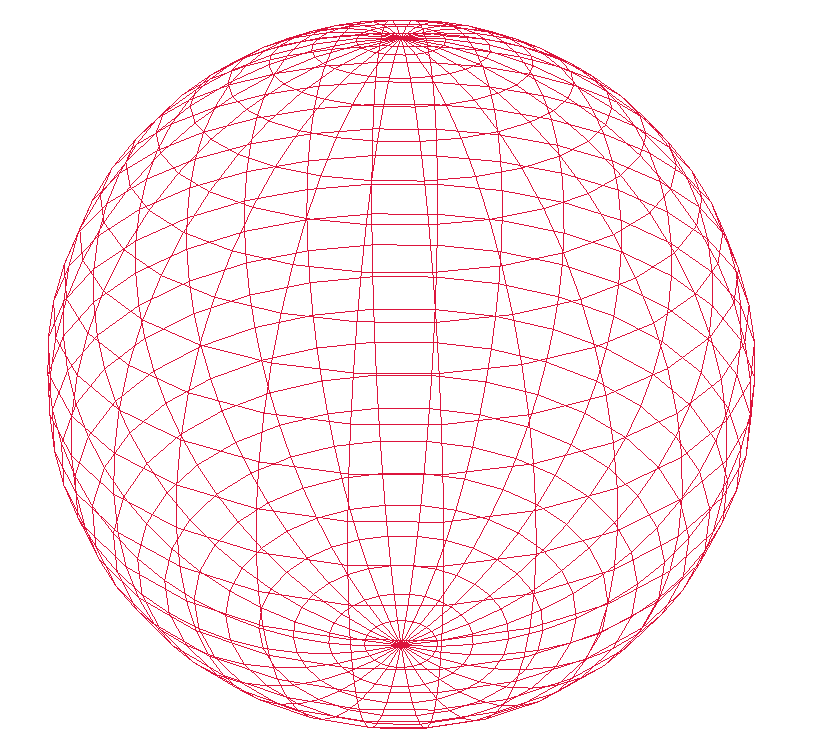
\includegraphics[width=0.4\linewidth]{sphere_vtk.png}\hfill
%   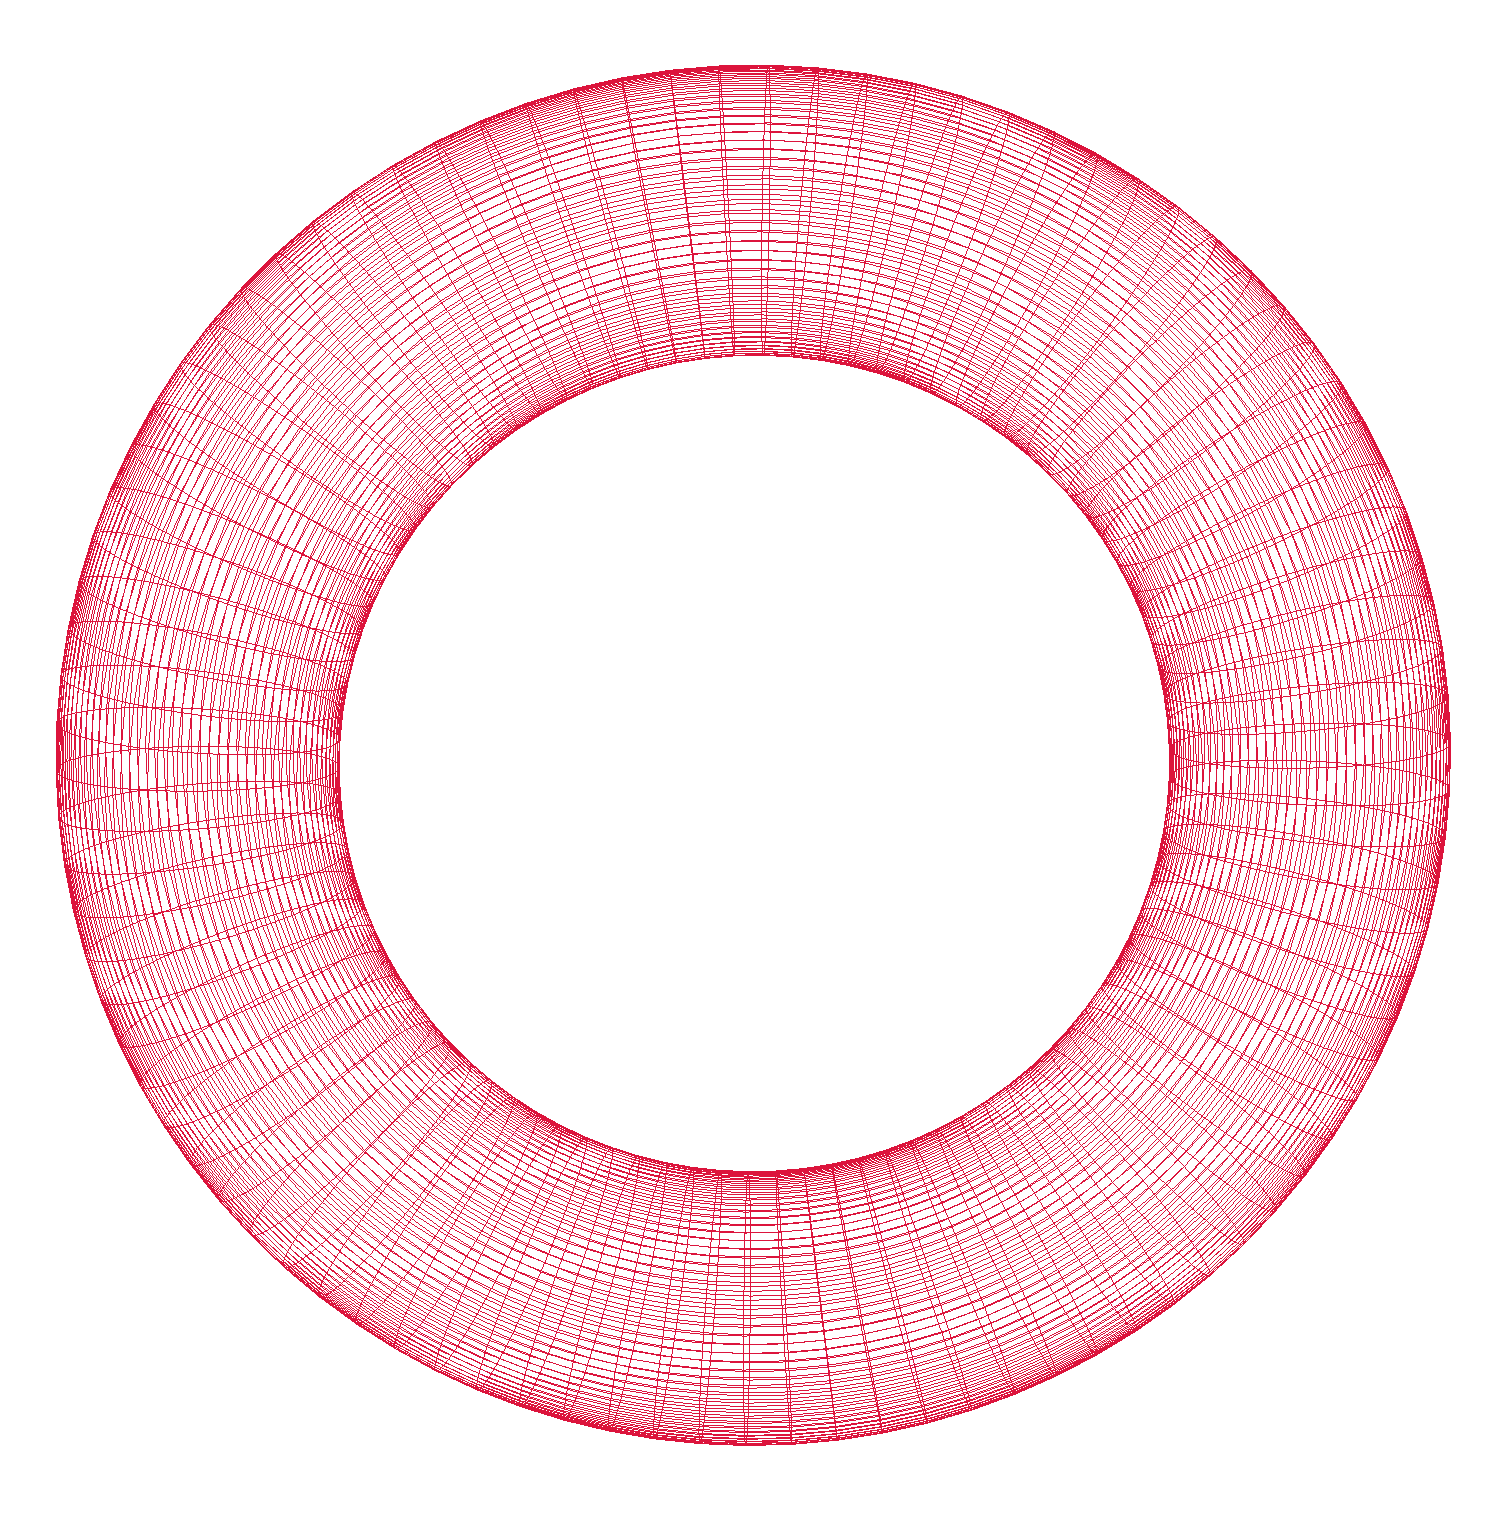
\includegraphics[width=0.4\linewidth]{torus_vtk.png}
%}
%
%\subsection{III/2 The twist vector}
%\frame{\frametitle{Mysterious twist vector}
%   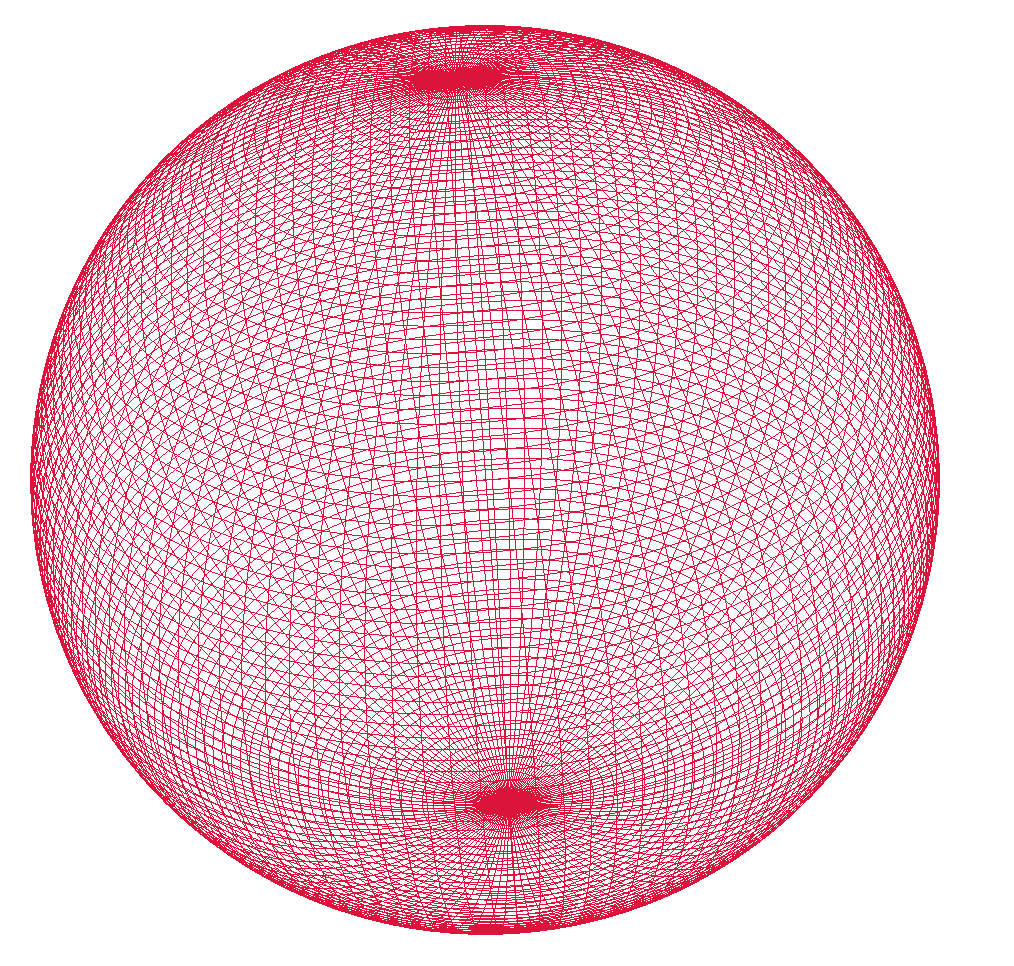
\includegraphics[width=0.5\linewidth]{sphere_twist.png}\hfill
%   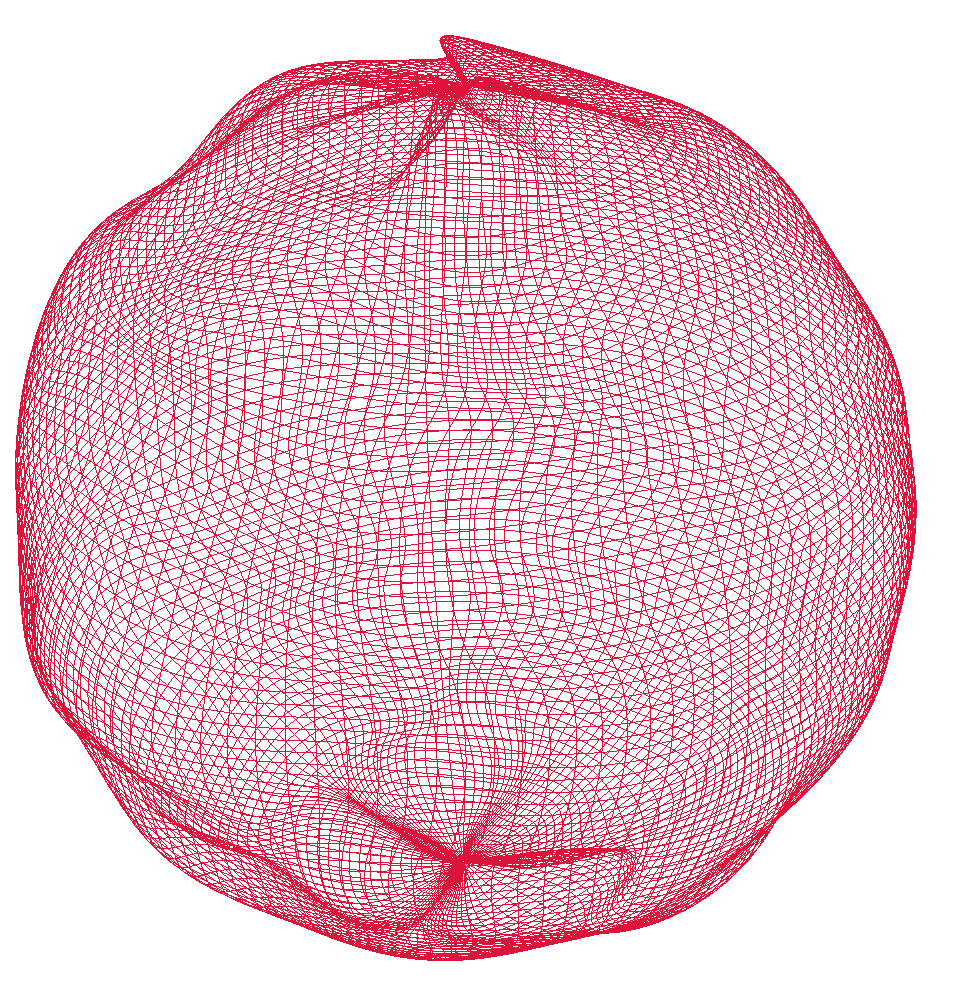
\includegraphics[width=0.5\linewidth]{sphere_twist_rand.png}
%}
%
%\section{Summary and future research}
%\frame{\frametitle{Summary and what next}
%  \underline{Take-away}
%  \begin{enumerate}
%       \item How to go from discrete to continuous
%       \item What are spline curves
%       \item What is a good basis
%  \end{enumerate}
%  \pause%
%  \underline{Ongoing}
%  \begin{enumerate}
%    \item Estimation of not intuitive parameters
%    \item Second-order Hermite interpolation
%    \item What basis for what purpose
%  \end{enumerate}
%}

\end{document}
